%\begin{abstract}
%The rapid urbanization process in the last century has deeply changed the way we live and interact with each other. As most people now live in urban areas, cities are experiencing growing demands for more efficient and sustainable public services that may improve the perceived quality of life, specially with the anticipated impacts of climatic changes. In this already complex scenario with increasingly overcrowded urban areas, different types of emergency situations may happen anywhere and anytime, with unpredictable costs in human lives and economic losses. In order to cope with unexpected and potentially dangerous emergencies, smart cities initiatives have been developed in different cities, addressing multiple aspects of emergencies detection, alerting, and mitigation. In this context, this article surveys recent smart city solutions for crisis management, proposing definitions for emergencies-oriented systems and classifying them according to the employed technologies and provided services. Additionally, recent developments in the domains of Internet of Things, Artificial Intelligence and Big Data are also highlighted when associated to the management of urban emergencies, potentially paving the way for new developments while classifying and organizing them according to different criteria. Finally, open research challenges will be identified, indicating promising trends and research directions for the coming years.
%\end{abstract}

%\begin{keywords}
%Smart cities, Emergencies management, Internet of Things, Sustainable cities, Resilient cities.
%\end{keywords}

%%% 1 %%%%%%%%%%%%%%%%%
\chapter{Revisão}
\begin{refsection}
\section{Introduction}

The development of new communication technologies, data processing algorithms, and cyber physical systems has not only transformed the way we gather information and interact with each other, but also how cities have evolved in the last decade \cite{smartcities1,smartcities7}. Affordable high-bandwidth communication networks and miniaturized hardware components with increasing processing power have become a reality, with deep but sometimes imperceptible impacts on the way we comprehend and handle different urban environments \cite{smartcities2,smartcities3}. For an increasing number of cities, smarter has become common sense \cite{smartcities8}.

The availability of new technological resources is expected to be a breakthrough for the development of sustainable, resilient, and smarter cities \cite{smartcities4}. By exploiting huge amounts of heterogeneous data, it is possible to better understand the multiple complexities of the urban environments, eventually leading to the implementation of ``smart services'' \cite{citiesvehicles,citiesdata,twitterDetection2}. Among them, emergencies management is expected to be a fundamental service in modern cities, with direct impact on urban safety and the perceived quality of life.

Generally speaking, emergencies have been an old and recurrent problem in cities, although their impact and influences have changed as cities grew larger \cite{emergenciesmetric1}. The spatial distribution of the cities and their geography through the centuries, as well as inherent characteristics such as poor sanitation, low mobility efficiency, dominance of wooden buildings, and the absence of rescue and emergency teams, have made cities highly susceptible to catastrophes resulted from emergency situations (the earthquake and fire on Lisbon in 1755 is a prominent example \cite{lisbon}). With the industrialization process and the further adoption of motor vehicles and telephone networks, emergencies management in modern cities improved, but actions were still dependent on emergency calls and non-automated dispatching of response vehicles \cite{fireevolution}. Currently, considering the new technologies available, more efficient solutions have been sought in order to minimize the negative impacts of emergencies.

When considering the construction of more resilient cities, research works in different areas such as Civil Engineering \cite{civilengineering1,civilengineering2}, Architecture and Urbanization \cite{architecture1,architecture2}, Environmental Sciences \cite{enviroment1,enviroment2}, Economics \cite{economics1,economics2}, and Sociology \cite{sociology1,sociology2} have contributed with models, discussions and valuable data to better understand the nature of emergencies, their immediate and long-lasting impacts, and the social and economical implications of emergencies on different populations in a city \cite{emergenciesmetric1,citiesemergencies1}. Although those research areas have given important perspectives about emergencies and their implications, technological developments have been crucial to handle urban emergencies, and they should be vital for the next generations of smart cities. In this sense, this article is specially concerned with the use of new technologies in the fields of Computer Science, Mathematics, Electrical Engineering and Telecommunications when addressing the detection and management of emergency situations in urban areas, surveying recent developments, and discussing open challenges and research directions. Doing so, we expect to provide a valuable reference for further investigations in this area, fostering the development of more sustainable and resilient cities. 

Emergencies can be better detected and managed with the use of electronic sensors, smartphones, personal gadgets, vehicles, drones, robots, social media networks, web servers, and could-based services. Usually, cyber-physical systems will be created to manage emergencies, processing data flows to provide one or more services in a city. In fact, such emergencies management systems will operate processing multiple types of data in a urban scale, which indeed is one of the fundamentals of the so-called smart cities paradigm \cite{smartcities4}. This is the conceptual background from where modern emergencies management systems have flourished.

Therefore, in order to make cities safer and more resilient, emergencies management systems have embraced different technologies to provide detection, alerting, and mitigation services in a city, automatizing different steps of the emergencies management cycle. However, since solutions have been developed following different approaches and premises, there is no consensus when addressing this problem, which may impair research and developments efforts in this area. Thus, a better understanding of this subject is desired. Figure \ref{Fig:general} depicts a general schema of an emergencies management system in a smart city with multiple detected emergencies, highlighting different sources of data.

\begin{figure}[htbp]
\centering
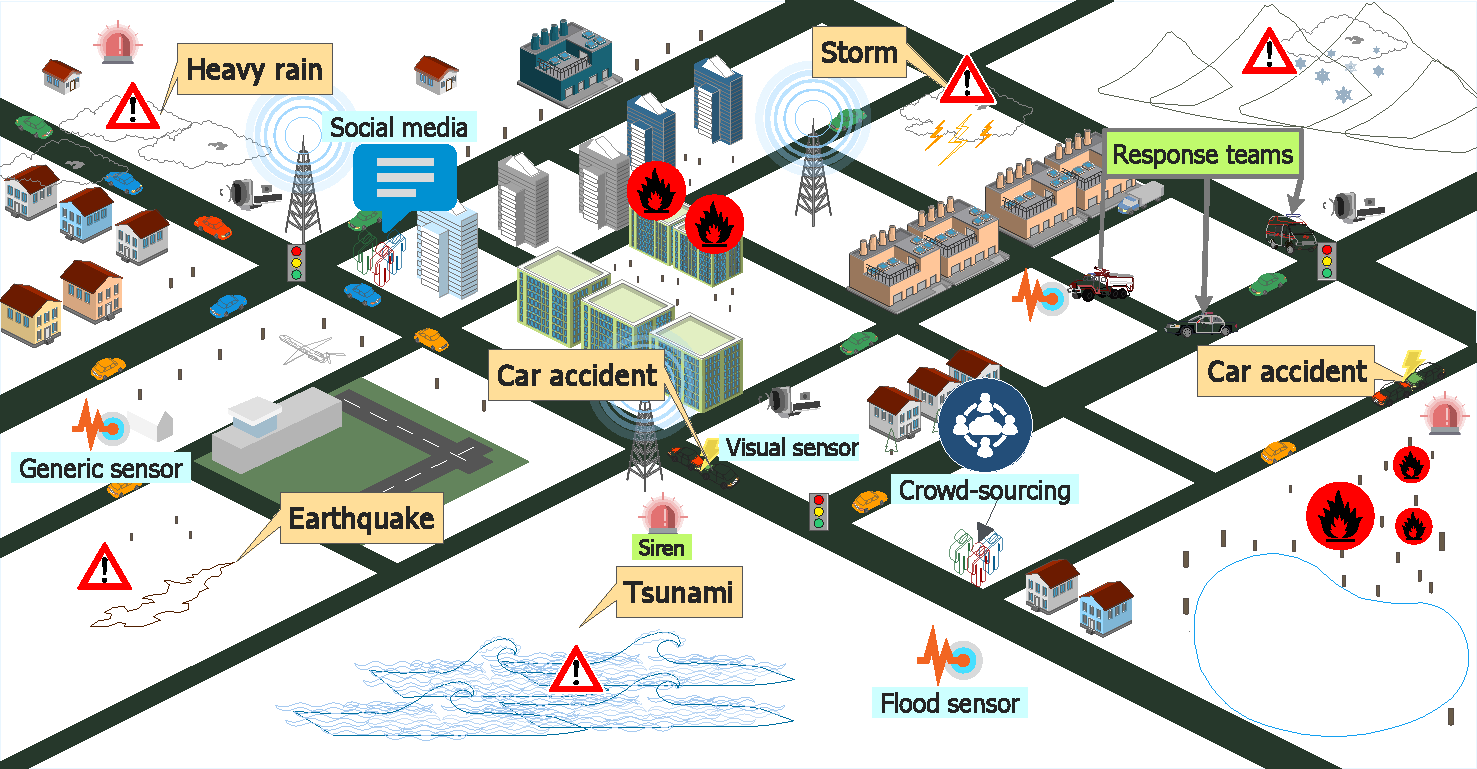
\includegraphics[scale=0.35]{Chapters/1-Survey/images/general.pdf}
\caption{Urban areas: a crisis-prone environment.}\label{Fig:general}
\end{figure}

The contributions of this survey are threefold. First, an emergencies management cycle is defined, classifying and organizing previous works according to their role on it. Second, the fundamentals of the area of emergencies management are established, comprising the concepts of hazards, emergencies, and alarms, which are discussed concerning their effect on the execution of the defined management cycle. Finally, previous works are surveyed and compared using as reference the provided definitions, allowing not only the understanding of the evolution of this area, but also giving clues about open challenges and research directions.

The remainder of this article is organized as follows. Section \ref{sec2} discusses the research context of this article, as well as the adopted methodology for the performed surveying. Section \ref{sec3} discusses the definitions and modelling of the emergencies management cycle and its defining elements. The current panorama of emergency detection is surveyed in Section \ref{sec4}. Section \ref{sec5} addresses alerting services that are executed due to the detection of an emergency. Section \ref{sec6} surveys mitigation actions that can be taken after one or more emergencies are detected in a city. Then, open challenges and research directions are envisioned in Section \ref{sec7}. Finally, conclusions and references are presented.

%%%%% 2 %%%%%%%
\section{Surveying emergencies in smart cities}\label{sec2}

Many aspects were considered when surveying the literature to achieve the expected results in this article. This section highlights the most relevant of such aspects.

%%%
\subsection{The smart service of emergencies management}

When considering the development of research works within the context of smart cities, some concerns may arise due to the nature of such environments. In recent years, smart cities initiatives have been proposed and implemented, embracing new technologies to enhance the citizens' quality of life, potentially making the urban living easier and bringing better management of its resources. Although such objectives seem to be clear, the number and types of complexities that emerge from smart cities initiatives are considerable, raising concerns that may echo and reach the development of emergencies management systems.

Much research efforts have been devoted to transform cities into smart cities \cite{citiestransforming,smartstrategy}. Since this is inherently a multidisciplinary area, researchers have tried to define best practices and engineering procedures to provide smart services in a city, taking into consideration development issues such as sustainability, social responsibility, and energy consumption \cite{citiestransforming2}. As a result, the literature in this area is diverse and potentially huge, covering different subjects comprising multiple views of the same urban environment.

In a typical smart city, several initiatives are devised to make citizens' life better and easier, improving several services such as public transportation, traffic management, water and energy supply, among others. In this sense, emergencies management systems arise as one of the possible services to be provided when defining smart cities, which may even coexist with other parallel services. Making the distinction of this service allow us to better define our scope of research, which will be adopted throughput this article.

At this point, it is worth to mention that although emergencies management systems will be considered in the performed surveying, only the technological aspects of their operations will be discussed. This is intended to help the readability of this article, without overlapping with existing literature in the area.

%%%
\subsection{Adopted surveying methodology}

In order to perform the intended reviewing about emergencies management systems, some criteria were defined. These were obtained from both the scope definition in previous subsection and the selection of some keywords to guide the intended surveying.

It was adopted the Scopus indexing database as reference, since it contains a significant part of the most relevant works in the considered areas, indexing both international journals and conference papers. For that, we adopted the following search queries:

\begin{description}
    \item[Search 1] TITLE-ABS-KEY ( ( "emergency response"  OR  "crisis management"  OR  "crisis model*" )  AND  "smart" )  AND  ( LIMIT-TO ( PUBYEAR ,  2021 )  OR  LIMIT-TO ( PUBYEAR ,  2020 ) OR  LIMIT-TO ( PUBYEAR ,  2019 ) OR  LIMIT-TO ( PUBYEAR ,  2018 )  OR  LIMIT-TO ( PUBYEAR ,  2017 )  OR  LIMIT-TO ( PUBYEAR ,  2016 ) )  AND  ( LIMIT-TO ( DOCTYPE ,  "ar" ) )
    
    \item[Search 2] TITLE-ABS-KEY ( "smart"  AND "emergency"  AND "response"  AND "management")  AND  ( LIMIT-TO ( PUBYEAR ,  2021 )  OR  LIMIT-TO ( PUBYEAR ,  2020 ) OR  LIMIT-TO ( PUBYEAR ,  2019 ) OR  LIMIT-TO ( PUBYEAR ,  2018 )  OR  LIMIT-TO ( PUBYEAR ,  2017 )  OR  LIMIT-TO ( PUBYEAR ,  2016 ) )  AND  ( LIMIT-TO ( DOCTYPE ,  "ar" ) )
\end{description}

In order to have the current picture of the state-of-the-art in emergencies management systems, a six-years window was considered for searching, from 2016 to 2021. The intention was to retrieve the newest relevant papers associated with the keywords \textit{emergencies response}, \textit{emergencies management}, \textit{crisis management}, \textit{crisis models} and \textit{smart cities}.

Considering ``Search 1'', it returned a total of 148 papers and ``Search 2'' returned 113 papers. For each search, title and abstract were manually analyzed to exclude non-related papers. After this filtering, only papers with an average of at least one citation per year were selected. Finally, duplicates were removed. Then, the resulting number of selected works was 51, which was assumed as the reference database when constructing the definitions for emergencies management systems and when comparing the proposed services for detection, alerting, and mitigation. Although a few works outside the defined criteria were eventually considered to support some arguments, all these 51 papers were the core reference for this article, being cited in proper sections according to their contents.

The workflow of the performed searches and papers selection is presented in Figure~\ref{fig:workflow}.

\begin{figure}[htb]
    \centering
    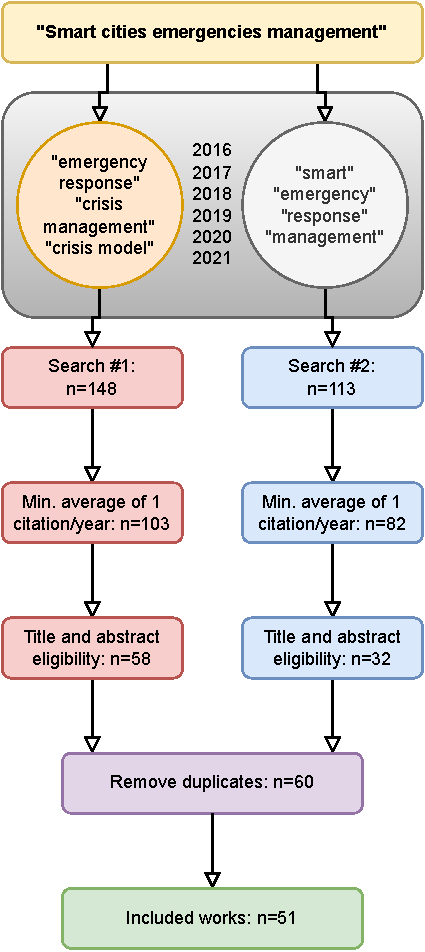
\includegraphics{Chapters/1-Survey/images/fluxograma.pdf}
    \caption{The adopted searching methodology for achieving the core set of works in this survey.}
    \label{fig:workflow}
\end{figure}

%%% 3 %%%%%%%%%%%%%%%%%
\section {The fundamentals of emergencies management systems}
\label{sec3}

The basic function of emergencies management systems in a smart city is the processing of conceptual emergencies along the time in response to detected critical situations. Such emergencies will typically be associated to the causes that created them, influencing the way how emergencies will be alerted and mitigated. Particularly, it is reasonable to say that emergencies will be associated to one or more causes (hazards), as well as to a group of additional information (metadata) that will give more details to support emergencies processing.  

Different methodologies and formalisms have been adopted in the literature when modelling and processing emergencies. However, there are some main characteristics that can be highlighted to better support the understanding of the evolution and current scenario of this research area. Among them, the logical definition of the concept of emergency is described in this section, as well as our proposed classifications for emergencies and emergency-based systems.

\subsection{The emergencies management cycle}

Although definitions may differ when considering the causes and the expected impacts, with some lack of consensus in the literature, it is reasonable to say that an emergency will be an indication of a dangerous situation, requiring proper and immediate action. This way, an emergency may be defined as the beginning of such dangerous situation, when cities may still do something to mitigate it in an attempt to reduce the probability of an emergency to become a disaster. Particularly, a disaster would be the worst consequence of an emergency in terms of inflicted damages, when cities can do little or nothing to mitigate its negative consequences. Hence, it is expected the development of smart city solutions to avoid or delay the occurrence of disasters, ideally diminishing their impacts when they become inevitable. 

Different approaches have defined procedures to handle emergencies and their impacts in urban areas \cite{citiesemergencies1,citiesdisasters1,emergenciesmetric2,mobilityEmergencies1,kumar2017emergency}. Actually, there are many similarities among previous works that allow us to define a generic processing cycle, which can be conceived in a broader concept referred as the ``management'' of emergencies. Such emergencies management cycle would initiate when hazards are perceived as emergencies. This happens when an emergencies detection service identifies that a hazard is being manifested, and this depends on how such service is configured. The detected emergency is then ``virtually'' issued along with all required metadata that is necessary to better understand the emergency and act properly. In the sequence, a notification (alerting/warning) procedure is initiated, informing to all affected and interested elements. Finally, this information processing flow goes to the execution of mitigation actions to cease the emergencies and relieve their impacts. 

Figure \ref{Fig:cycle} depicts this overall emergencies management cycle in smart cities. 

\begin{figure*}[htbp]
\centering
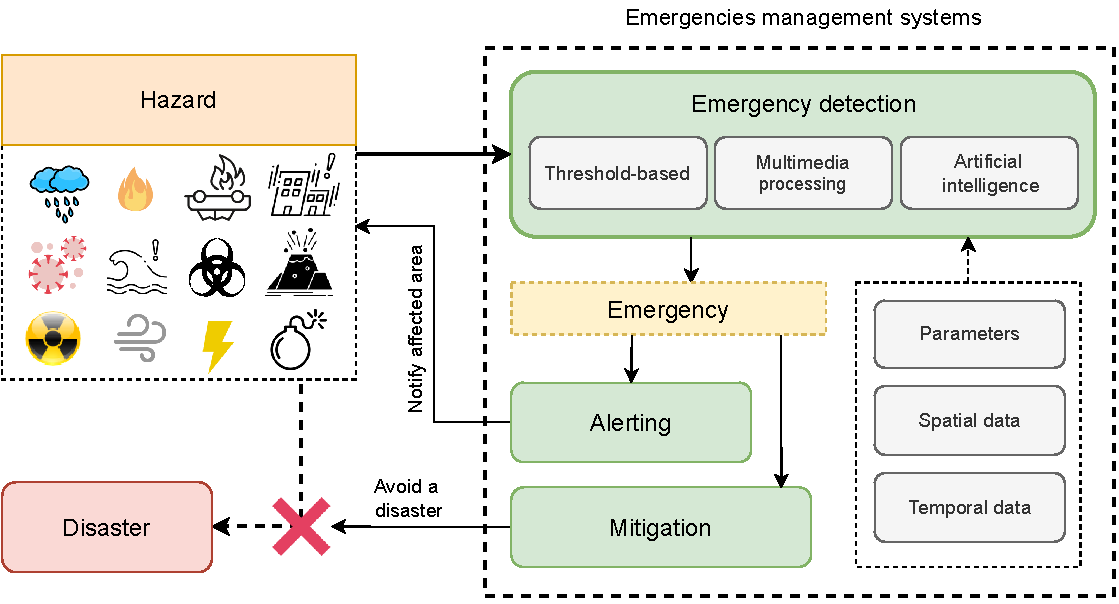
\includegraphics[scale=0.85]{Chapters/1-Survey/images/newcycle.pdf}
\caption{The emergencies management cycle: a hazard is perceived as an emergency to support alerting and mitigation actions.}
\label{Fig:cycle}
\end{figure*}

We consider the following definitions for the elements that compose the proposed emergencies management cycle, described as follows:

\begin{itemize}
    \item \underline{Hazard}: It is the inherent source of danger in an urban environment. In other words, a hazard is a potential cause of a critical situation that may have negative consequences on a city. The hazards will have different origins and behaviors, with different occurrences depending on geographical characteristics and urbanization patterns \cite{hazard1,hazard2}. Although they are the original cause of a disaster, hazards may never happen in a city, while other cities may experience constant critical situations resulted from a single threat \cite{hazard3}. Therefore, in order to properly detect emergencies, hazards have to be continuously monitored;
    
    \item \underline{Emergency}: It is the key element that defines that something is wrong and that something has to be done about it. Usually, an emergency will be a conceptual element that exists within computer-based systems, being created when a hazard is perceived as a current menace and it is detected by some means \cite{socialmedia1,citiesdisasters1}. The objective of an emergency is to provide helpful information to guide the required actions to avoid harmful consequences in a city \cite{emergenciesgeneral1};
    
    \item \underline{Disaster}: It is the ultimate consequence of an emergency that was not tackled by an emergencies management system on time. It is expected that smart cities will treat emergencies in a way that disasters are avoided and thus this is the primary objective of emergencies management systems. However, when untreated emergencies become disasters, some specialized solutions may still be employed, and there are many works in the literature that have addressed particular problems of pre- and post-disaster scenarios \cite{citiesdisasters1,citiesdisasters2};

\end{itemize}

This article is particularly concerned with smart city solutions to handle emergencies before a disaster happens. For that, the defined emergencies management cycle highlights three major processing steps: detection, alerting, and mitigation. All these steps will be discussed in details, as well as the conceptual definitions of emergencies in the literature, encompassing all their complexities. 
%%%%%

%%%
\subsection {Hazards}

In a urban environment, a hazard is any source of potential damage that may harm people or incur in economic losses when it becomes an emergency. Usually, a hazard is perceived as an emergency when it is a current threatening condition, and it ceases to exist when it represents no more risks. This way, for example, the temperature hazard will only become an emergency when it is higher than a safety threshold, or when it is perceived as critical when combined with other hazards. The proper modelling of the hazards is then of paramount importance for this type of applications.

The most usual approach to model and process hazards is to monitor a particular variable along the time. Actually, such approach is easier to implement and may produce very quick responses when employing electronic sensor devices or active data sources. Differently, hazards may be also processed as more complex variables, for example employing cameras \cite{emergenciesmetric3} or artificial intelligence algorithms \cite{emergenciesAI1} to detect hazards that could not be easily identified using individual sensors, generating different types of emergencies. As an example, a fire event could be identified processing still images or processing public posts on social media, potentially providing different types of metadata to support emergencies mitigation actions. Whatever the case, each system will have a particular configuration for hazards monitoring and emergencies detection, according to the characteristics of the target city.

Since the nature of a hazard will dictate how an emergency will be eventually mitigated in a urban environment \cite{citiesdisasters1,hazard2,hazard4}, city-related hazards may be classified into three different groups: Environmental, Urban and Health. Environmental hazards are those resulted from natural conditions that may affect a city, such as heavy rain, hurricanes, earthquakes, volcano eruptions, among others. The other two types of hazards, Urban and Health, are both causes of human-induced disasters. We propose to subdivide them into two different groups due to the expected relevance that outbreaks surveillance and detection systems should assume in the development of smart cities \cite{covidsmartcities1,covidsmartcities2,enviroment3}. This way, Urban hazards will be related to the way we live in cities, with increasing overpopulated areas and crowded mobility systems, resulting in hazards related to traffic accidents, house firing, gas explosion, building collapsing, terrorist attacks, violent protests, robbery, etc. Finally, Health hazards will not only be associated to individual health emergencies, such as heart attacks, but collective threats due to the spread of infectious diseases. Figure \ref{Fig:hazards} presents a comprehensive organization of the expected hazards in urban areas. 

\begin{figure*}[htbp]
\centering
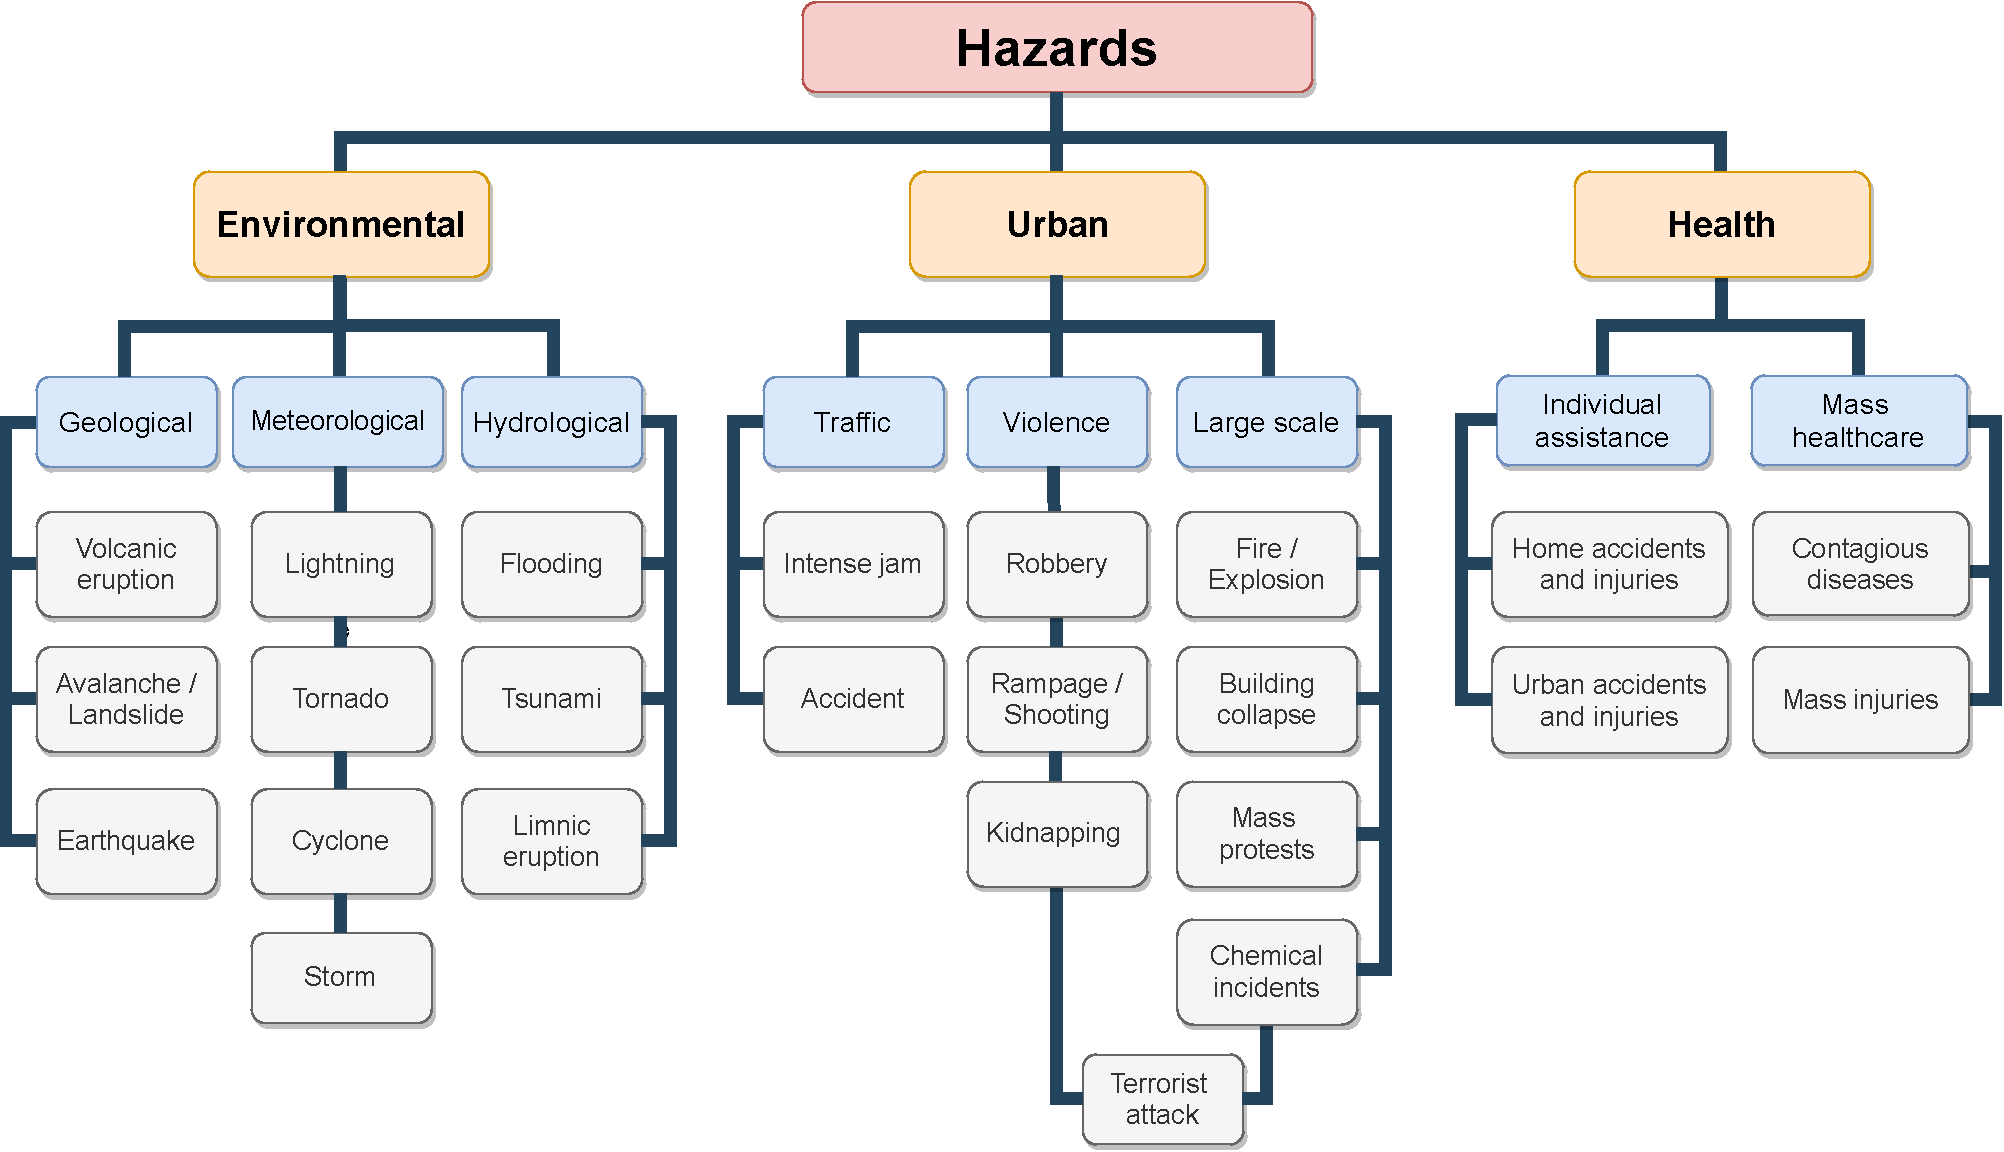
\includegraphics[width=\linewidth]{Chapters/1-Survey/images/Hazards.pdf}
\caption{The proposed classification and some common hazards in modern cities.}
\label{Fig:hazards}
\end{figure*}

Human-induced disasters may result in infrastructural damages, injuries and deaths. Although there is not a straight line between the frequency of Urban and Health hazards and the urbanization process, the urban sprawl in this century will result in more large and mega cities around the world, with potential for higher number of disasters \cite{urbansprawl1,urbansprawl2}. In parallel, climate changes are strengthening the destructive power of natural disasters, putting additional pressure on emergencies management systems \cite{enviroment1,enviroment2}. As a result, the last decades have seen an increasing in the number of emergencies detection approaches, focusing on different types of hazards. 

%%%%
\subsection{Defining and modelling emergencies}

Emergencies are defined as a virtual entity that comprises one or more hazards and a group of metadata. Hence, for emergencies detection systems, a major issue will be to define how coupled are the emergencies concerning their associated hazards, which lead us to propose two different classifications for the definition of emergencies:

\begin{itemize}
    \item \underline{Self-contained emergencies}: Since emergencies are critical situations that may cause damages, injuries and deaths, many approaches have focused on handling them as self-contained critical elements. In such cases, an emergency is associated to a single hazard, resulting in emergencies being a result of a single cause. This way, for example, there are Earthquake Emergencies, Fire Emergencies, Flooding Emergencies and Traffic Emergencies. For some solutions targeted at a single type of emergency, such as the work in \cite{iotFire1} for fire emergencies and the work in \cite{iotRain1} for heavy rain emergencies, the proposed system is usually deployed to detect a particular type of hazard. Differently, other approaches provide some level of flexibility, allowing the detection of different hazards, but the eventual issue of an emergency is still associated with a specific type of hazard, as in \cite{emergenciesmetric4}. Whatever the case, the processing of self-contained emergencies (also referred as atomic emergencies \cite{emergenciesmetric6}) has been adopted as a simpler way to issue and handle emergencies that have the characteristics of their single associated hazards;
    
    \item \underline{Events-based emergencies}: For some systems, each manifested hazard will be processed as individual critical events, which will be independent indications that something critical is happening or about to happen. In this perspective, an emergency will be the conjunction of one or more events, acting then as a ``container'' of manifested hazards. For such systems, the separation between events and emergencies allow a more structured processing of critical situations, since emergencies can be defined as a composition of multiple critical events that may give more detailed clues about what is happening at a certain place and time.
\end{itemize}

Since events-based emergencies may be too complex when considering all the possibilities in smart city scenarios, we also classify it into two different subgroups, defined as follows:

\begin{itemize}
    \item Triggered emergencies: It happens when thresholds are exploited to trigger the detection of an emergency. Overall, this is a simpler way to detect emergencies, since thresholds can be defined for a group of hazards monitored by sensors or other data source. In \cite{emergenciesmetric2}, an event of interest is associated to a scalar metric measured by a sensor, and each event of interest is triggered when the measured values are higher (or lower) than defined thresholds. Then, all triggered events are used to compose a single emergency. As an example, for a temperature threshold of $50^{\circ}$C, an emergency is detected when the measured temperature is higher than that reference value, but other types of hazards may also compose the same detected emergency;
    
    \item Aggregated emergencies: For a particular group of emergencies management systems, emergencies will be detected not by triggering and safety thresholds, but by the combined processing of multiple monitored hazards. In these cases, multiple hazards are monitored and considered for the detection of emergencies, in a combined way, creating either separate emergencies or combined macro-events emergencies, depending on the characteristics of the implemented system. For such group of emergencies, multimedia processing algorithms and artificial intelligence can be employed to combine multiple data from monitored hazards, exploiting techniques and algorithms in areas such as visual computing, audio processing, machine learning, genetic computing and fuzzy logic. The work in \cite{SultanMahmud2017} makes use of machine learning algorithms to read several sensors and generate a fire danger level instead of just monitoring thresholds. Images of the monitored area are also interpreted by machine learning algorithms to better define if there is a fire emergency or not. Another relevant scenario for such type of processing and modelling is the early detection of emergencies using machine learning, when the combined perception of the behavior of the expected hazards indicate that something may soon become wrong \cite{machine1}. Such solutions could be even exploited to support a different class of applications in the area of emergencies avoidance, as already largely adopted for traffic avoidance in Intelligent Transportation Systems (ITS) \cite{machine2}.
\end{itemize}

It is important to notice that hazards are the original causes of emergencies, thus indicating their nature. This way, for example, an emergency issued due to a temperature hazard may suggest the dispatching of fire trucks, while an emergency issued after a traffic accident may be handled by adjusting traffic lights. Therefore, understanding the possible hazards in a city is crucial when managing emergencies. 

Table \ref{Tab:hazards} summarizes some works in the literature concerned with emergencies, highlighting their characteristics according to the modelling of hazards.

\begin{table*}
\centering
\caption{Research works and the modelling of hazards and emergencies.}
\label{Tab:hazards}
\begin{tabular}{|c|c|c|c|c|c|c|c|}
    \multirow{2}{*}{\textbf{Work}} & \multirow{2}{*}{\textbf{Year}} & 
    \multicolumn{3}{|c|}{\textbf{Hazards}} & \multicolumn{3}{|c|}{\textbf{Emergencies}}\\
    \cline{3-8}
    & & Environ. & Urban & Health & Self-contained & Triggered & Aggregated \\ 
    
    \hline
    \citeauthor{emergencyTraffic1} \cite{emergencyTraffic1} & 2012 &  & vehicular sensors & & X & & \\
    
    \hline
    \citeauthor{detectionAudio1} \cite{detectionAudio1} & 2013 &  & audio & & X & & \\
    
    \hline
    \citeauthor{iotRain1} \cite{iotRain1} & 2016 & rain &  &  & X & & \\
    
    \hline
    \citeauthor{SultanMahmud2017} \cite{SultanMahmud2017} & 2017 & fire & fire & & & & X \\
    
    \hline
    \citeauthor{iotDetection2} \cite{iotDetection2} & 2017 & multiple data & multiple data & multiple data & & X & \\
    
    \hline
    \citeauthor{iotDetection1} \cite{iotDetection1} & 2018 & multiple data & multiple data & multiple data &  & X & \\
    
    \hline
    \citeauthor{iotFlood1} \cite{iotFlood1} & 2018 & water & water & & X & & \\
    
    \hline
    \citeauthor{iotFire1} \cite{iotFire1} & 2018 &  & gas, smoke, temperature & & X & & \\
    
    \hline
    \citeauthor{iotPollution1} \cite{iotPollution1} & 2019 & air pollution & & & X & & \\
    
    \hline
    \citeauthor{Alkhatib2019771} \cite{Alkhatib2019771} & 2019 & & multiple data & & & & X \\
    
    \hline
    \citeauthor{BRAGAGNOLO2020104240} \cite{BRAGAGNOLO2020104240} & 2020 & landslide & & & & & X \\
    
    \hline
    \citeauthor{emergenciesmetric2} \cite{emergenciesmetric2} & 2020 & multiple data & multiple data &  multiple data &  & X & \\
    
    \hline
    \citeauthor{emergenciesmetric3} \cite{emergenciesmetric3} & 2020 & multimedia data & multimedia data & multimedia data &  & X &\\
    \hline
    
    \citeauthor{iotCovid1} \cite{iotCovid1} & 2020 &  & visual data &  & X & & \\
    \hline
    \citeauthor{iotEarthquake1} \cite{iotEarthquake1} & 2020 & earthquake &  &  & X & & \\
    \hline
    
    \citeauthor{twitterDetection1} \cite{twitterDetection1} & 2020 & social media & social media &  social media &  & X & \\
    
    \hline
    \citeauthor{fireBigdata1} \cite{fireBigdata1} & 2021 & fire & fire & & & & X \\
    
\end{tabular}
\end{table*}

%%%%%%%%%%%%
\subsection {Associating metadata to the emergencies}

When an emergency is detected within an emergencies management system, it is virtually created to be further processed. Such emergencies will be typically associated to a group of metadata, providing different types of information. Although there may be different types of metadata associated to emergencies, we identified three major groups that will be mostly considered when handling emergencies, defined as follows.

\subsubsection{Affected area}

An emergency will usually be assumed to occur in the same area of its cause (one or more hazards), which is defined as its ``area of incidence''. This is usually a point on a city that may be located on public or private areas, depending on the adopted approach and the monitored hazards. Actually, although it may be reasonable to use relative positions in a urban environment, or even Cartesian coordinates according to a reference point, many approaches will employ GPS (Global Positioning System) coordinates to precisely locate the areas of incidence of detected emergencies. Actually, the adoption of GPS coordinates has led many approaches to exploit sensor units equipped with GPS devices \cite{smartsensing1} or to use GPS-enabled smartphones when harnessing crowdsourcing algorithms \cite{smartsensing2}.

In fact, the location of the detected hazards will be the reference position of the corresponding emergency, but some approaches may also assume that an emergency will be felt in an area irradiating from that location. That ``influence zone'' may be modelled in different ways, although it will be often processed as a circular area with the area of incidence as the center of that circumference \cite{s150614370}. Additionally, as an important remark, two different hazards may be associated as belonging to the same emergency if they are being detected within a certain area not greater than some defined tolerable distance. Obviously, it will be a function of the desired precision, since two different hazards detected in the same block or street could be processed as the same emergency for practical reasons.

It is worth to mention that a wider influence zone may be defined according to the type of the detected hazard and the affected area. For example, a fire hazard in a neighborhood with many wooden houses may be too critical because the fire may rapidly spread, specially under windy conditions (which may be also processed as a hazard) during a dry season (a temporal significance of the emergency, as further discussed in this article) \cite{iotFire2}. In such cases, the initially detected emergency may have a wider influence zone, for example allowing preventive evacuation \cite{evacuation}.

%%%%%%%
\subsubsection{The duration of emergencies}

Since all emergencies will be associated to at least one hazard, a particular emergency is issued when an associated hazard is considered to be manifested in an area, either because a corresponding event was triggered or due to some aggregated processing of multiple hazards. Whatever the case, although the cause of an emergency may rapidly cease, for example in an earthquake, its effects may endure for a longer time, threatening people in different ways. For example, the impacts of an emergency composed of both earthquake and tsunami hazards may be sensed for days or weeks, even if those hazards persist in a critical level for just a few minutes \cite{tsunami1}. This way, emergencies management systems should be aware that emergencies may have different temporal behaviors, which may be affected by the type of hazards and by the social, economical and spatial characteristics of the considered city.

Actually, there is a gray area in the literature considering how critical situations persist in a city. In some perspectives, a critical situation that last for some time may be considered as a pre-disaster  
period \cite{citiesdisasters2,citiesdisasters3} or even a post-disaster situation \cite{citiesdisasters4,citiesdisasters5}. On the other hand, the duration of a critical situation may roughly be the duration of an emergency that can still be addressed before a disaster is formally defined, as expressed in the management cycle in Figure \ref{Fig:cycle}. Although there is not a consensus about the temporal significance of emergencies and disaster configurations, this article is mostly concerned with the duration of emergencies that can still be mitigated by some computer-assisted system.  

Therefore, for many emergencies detection approaches, an emergency will last for some time even after the original hazard stop being critical, benefiting mitigation actions as the assignment of emergency response teams. For the work in \cite{emergenciesmetric2}, that duration depends on each mitigation approach, which could assume any duration after an emergency stop being reported. Also, an algorithm is proposed in that work to model a temporal significance of emergencies that slowly decreases over time, which may be quite realistic for some types of hazards. In other perspectives, such as in \cite{socialmedia1,emergenciesmetric4,emergenciestimemedia}, emergencies can be assumed as active as long as their causing hazards are being perceived as critical. The modelling of the duration of emergencies is then an important project characteristic, with a lot of practical implications.

%%%
\subsubsection{Computing severity levels} 

Emergencies will be detected at a certain position, having an influence zone and lasting for some time. Although all this metadata is relevant to understand and to model emergencies, their real potential to cause destruction, injuries and deaths may rely on other types of parameters. Actually, such potential of destruction, generically measured as the ``severity level'' of an emergency, may be a function of many variables besides the hazards that created it.

In general, we can expect that self-contained emergencies will rely on the magnitude of the monitored hazards, while events-based emergencies would exploit other types of information to indicate their level of criticality. Considering the proposed approaches in the literature, in different scopes, we have identified different groups of parameters to be used when computing a severity level for the emergencies, which are summarized as follows:

\begin{itemize}
    \item Hazard significance: Since emergencies will be associated to one or more hazards, it is natural to compute the severity level based on the characteristics of the hazards that compose them. However, there are different characteristics to be accounted, resulting in different ways to compute such level. For threshold-based approaches, hazards are processed as ON/OFF events and thus the severity level is only impacted by the number of triggered events that compose the considered emergency \cite{emergenciesmetric2}, or simply by the manifestation of the hazard itself \cite{emergenciesmetric4}. In such cases, a hazard is already something critical, and there is no hazard that is more critical than other hazard of the same type \cite{emergenciesmetric2}. On the other hand, the ``intensity'' of a hazard may also impact the criticality of an emergency, and two temperature hazards originated from different sensed temperatures will account differently when computing the severity level;
    
    \item Spatial significance: The areas of incidence and the influence zone are useful information to indicate where mitigation procedures can be taken to save lives and reduce damages. That information may be already present as metadata of emergencies and thus it seems natural to exploit them to enhance the computation of the severity level. In fact, the potential of negative impacts may be a function of the area under an emergency in a city, and different parameters may be considered for that. Actually, the inherent risk of damages in an area may be accounted based on the 1) the spatial composition and organization of the buildings and infrastructure, and 2) the population density and mobility patterns in a city. For example, an area with many wooden houses may have an innate risk \cite{firespatial1} and thus a fire emergency in such a region should be more critical for a city as a whole \cite{firespatial2}, potentially leading to the necessity of some prioritization when dispatching fire trucks to attend that emergency \cite{costa2020automatic}. In a different perspective, areas with high population density in large cities may also suffer more from the same emergency when compared to low populated areas in the suburbs \cite{firespatial3}. Since such population density may vary along the time, according to urban mobility patterns \cite{mobilityEmergencies1}, it is also reasonable to apply dynamic mechanisms to compute the severity level according to how people move within a city;

    \item Temporal significance: The third element that might be accounted when computing the severity level is the temporal significance associated to the affected area. Actually, when an emergency is happening is very important since its negative effects may be boosted or attenuated according to movement patterns and the availability of mobility services along the days, weeks and months. In this sense, holidays and weekends may impact the emergency severity level, as well as hush hours in weekdays. In \cite{firetemporaldata1}, statistical analysis of fire concerning the time of the day, the day of the week and the month of the year are performed, associating temporal data with the impact of fire hazards. For the work in \cite{hurricanetemporal1}, multiple data are combined to estimate the impacts of hurricanes, predicting their trajectory. Then, other emergencies in a city would have higher levels of criticality if they occur during a hurricane season. In other example, crime incidents during the day, night and dawn could be used to classify emergencies \cite{crimetemporal1}, specially when related with urban hazards. In all these cases, temporal modelling would provide additional data to support the assessment of the severity level of the emergencies.

\end{itemize}

There are important remarks when computing the severity level of emergencies and the literature has presented interesting solutions when handling them. In general, it is reasonable to say that the monitored hazards and the expected outcomes of the employed systems will strongly dictate how severity will be computed. For the work in \cite{iotEarthquake2}, multiple sensors are used to gather information about acceleration and vibration, which is used to detect earthquakes. A warning message (emergency) emitted by that system is classified into one of three different levels, according to the detected shaking intensity. However, a different approach would be to assume that any earthquake with a magnitude higher than a certain threshold would already be a critical situation. For the work in \cite{iotEarthquake3}, a sensor network is used to detect earthquake emergencies, which are issued when a seismic peak is detected. In that case, all hazards have the same severity level. But since the hazard is an earthquake, it is already a threatening condition and thus giving a severity level to it may be pointless for some applications (a detected earthquake is already bad enough when it is higher that a ``safety'' level).

Another interesting remark is that the definitions of the impacts of spatial metadata of an emergency may vary considerably, depending on the developed system and the target city. In this sense, a downtown area with many hospitals and schools may be more severely affected by the same type of emergency in the suburbs, but the other way around is also possible if there are critical chemistry industries at the suburbs. The lack of efficient mobility may also impact emergency vehicles, which would be dispatched from some fixed stations (e.g. a fire department). In fact, such spatial significance may be not easy to be defined, demanding proper modelling.

It is also worth saying that some types of hazards are hard to graduate within a scale. In a traffic accident, for example, it may be meaningless to account the number of involved cars, since the number of victims may be a more desired information to be considered. The same reflections can be made for other urban or health hazards. Actually, many emergencies systems related to such hazards have implemented crowdsensing approaches to detect them, which make it hard to compute severity levels based on the hazard nature. Particularly, it is better to classify all these emergencies as equally critical, relaying on other parameters to compute levels of criticality. In \cite{emergenciesmetric3}, the severity level of events-based triggered emergencies is a direct function of the number of detected hazards. However, since there are some hazards that may provide more information about a particular critical situation, that work assigns twice the relevance for hazards detected using cameras and visual processing algorithms, when compared to hazards detected by scalar sensors. For example, if a building is on fire, a camera may detect a fire emergency which is twice as relevant as temperature or smoke emergencies. Nevertheless, in that work, all emergencies resulted from the same type of cause (hazard) will still have the same impact on the severity level, regardless of their sensed intensity or magnitude. 

The final objective of giving an impact level to the emergencies is to support decision algorithms when handling multiple concurrent emergencies. Since many cities may have finite resources to attend emergencies, for example concerning the availability of emergency vehicles and response teams \cite{costa2020automatic,tsunami1}, such severity assessment may be an important element for emergencies management systems. Once again, each city may have particular temporal and spatial significance, which may be associated with its sub-regions and neighborhoods. Therefore, proper modelling of such characteristics would be worth when computing all metadata related to emergencies in a city, improving the effectiveness of the employed systems and the alerting and mitigation procedures.

%%%%%%%%%%%%%%%%%%%%%%%%%%%%%%%%%%
%%% 4 %%%%%%%%%%%%%%%%%
\section{Detecting emergencies}
\label{sec4}

When reviewing previous works in the research area of smart emergencies management, particularly when concerning to the detection of emergencies, it is possible to sort out three major sources of data: sensors, crowdsourcing and big data. Sensors will be used to directly monitor one or more hazards, as close as possible to the affected area. Crowdsourcing will use a different paradigm, indirectly collecting data from multiple sensors, gadgets and even people to perceive a critical situation. Finally, big data approaches will usually process data from multiple sources not necessarily related to the monitored hazards, even considering data of historical occurrence of emergencies in an area. 

The detection of emergencies may then be performed in multiple ways and the literature has also presented some interesting solutions about the detection and the issuing of emergencies exploiting very different data sources. Actually, although such sources may differ concerning characteristics as availability, scalability, cost and accuracy, it is usually expected the definition of at least one Emergencies Detection Unit (EDU) to perform detection functions, even in a more generic way, which will have a well-defined data input, one or more processing algorithms and some additional configurations for the emergencies (metadata). EDUs may be implemented on electronic components ``on the edge'' (closer to the hazards) \cite{PlatformsSC,sensorsplatforms}, on central computers \cite{twitterDetection2,centralserver1} or even exploiting cloud-based services \cite{cloud1}, either taking a single input data stream or having multiple data sources at once. 

Figure \ref{Fig:detection} depicts a generic scheme for the detection of emergencies in smart cities. 

\begin{figure}[ht]
\centering
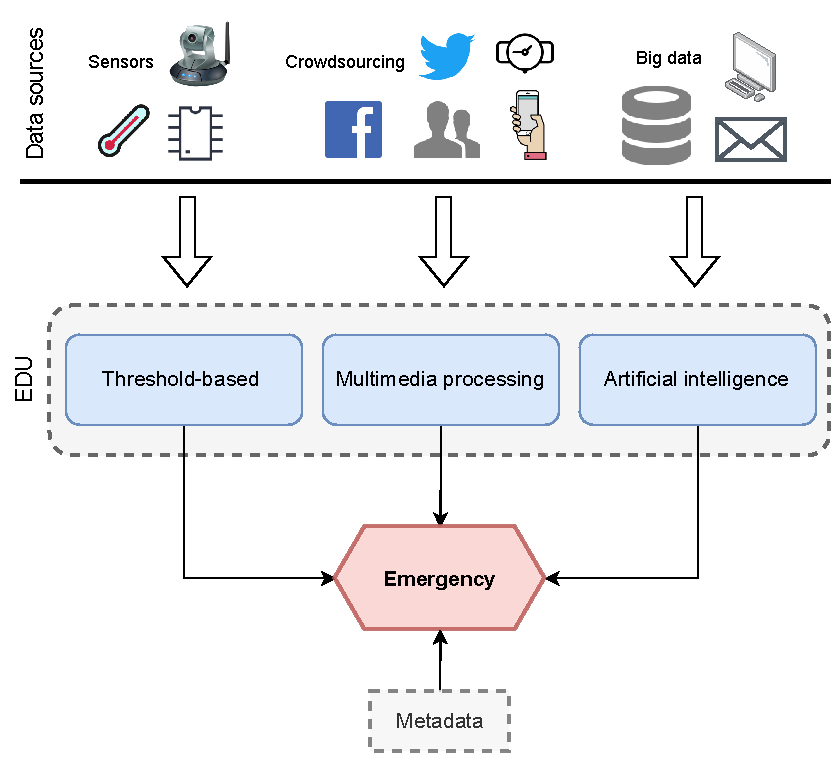
\includegraphics[scale=0.6]{Chapters/1-Survey/images/detection.pdf}
\caption{Detecting emergencies through the monitoring of hazards in a city, considering different sources of data.}
\label{Fig:detection}
\end{figure}

%%%
\subsection{Input data sources}

The detection of emergencies should exploit different sources of data in order to take more accurate decisions. However, characteristics of the employed approaches and the particularities of the target city will dictate the best (and more affordable) data sources to be considered. Therefore, in order to better understand how they could be used in practical applications, the three major sources of data for emergencies detection are discussed in next subsections.

%%
\subsubsection{Electronic sensors and sensor networks}

The most direct way to detect emergencies is to employ sensor devices to monitor a particular hazard along the time. Such electronic components are able to measure a particular variable, which can be processed locally \cite{edge1} or transmitted to other devices for further processing \cite{iotRain1}. Additionally, while sensors may be exploited to detect a specific group of hazards (fire, pollution, rain, flooding, gunshots, etc), it is also possible to employ them to support adjustable architectures to monitor any groups of hazards and emergencies \cite{emergenciesmetric2,emergenciesmetric4,emergenciesmetric6,emergenciesmetric5}. Whatever the case, sensors will provide scalar or multimedia data to be further processed by any detection algorithms.

When implementing the generic concept of an EDU, sensors may be attached to an electronic processing board that will handle all sensing activities, as well as the networking and data processing functions expected from it. Such boards may have a continuous energy supply or they may be powered by batteries \cite{energy1}, affecting the deployment planning of the EDUs and their mobility patterns. In fact, the proper choosing of the hardware and software characteristics of the employed sensors and the associated central processing unit has proven to be an important project decision of computer-assisted solutions for emergencies detection, with important developments in recent years \cite{sensorsplatforms,sensorsplatforms2,sensorsplatforms3}.

The use of sensors to detect emergencies has maturated along with the evolution of Wireless Sensor Networks (WSN) \cite{surveywsn2}. Since the beginning of WSN developments, sensors had being harnessed to monitor critical zones as factories, furnaces, nuclear reactors and several equipment that could bring danger to people and nearby facilities. With the emerging concepts of Internet of Things (IoT) and smart cities, sensors are now perceived in a broader perspective that comprises virtually anything in a urban environment \cite{smartsensing1,smartsensing3}. This flexibility, together with the increasing affordably of powerful electronic boards for open source and open hardware developments \cite{PlatformsSC}, have not only transformed the way smart cities have been created, but also how emergencies can be better managed on modern cities. Therefore, the adoption of sensors-based emergencies detection units is the culminating point of a continuous evolution process. 

Table \ref{Tab:sensorsbased} summarizes previous works in the literature that employ one or more sensor devices to support the detection of emergencies.

%% Table
\begin{table*}
\centering
\caption{Sensors-based detection of emergencies.}
\label{Tab:sensorsbased}
\begin{tabular}{|c|c|c|c|c|}
    \textbf{Work} & \textbf{Year} & \textbf{Hazard} & \textbf{Sensors} & \textbf{Processing hardware}\\

    \hline
    \citeauthor{iotRain1} \cite{iotRain1} & 2016 & rain & air pressure, temperature, humidity, wind speed, solar & Raspberry Pi 2 \\

    \hline
    \citeauthor{iotRain2} \cite{iotRain2} & 2016 & extreme weather & air pressure, humidity, wind speed and direction & Arduino Uno \\
    
    \hline
    \citeauthor{iotFire4} \cite{iotFire4} & 2017 & fire & smoke, gas, flame & ESP 32\\
    
    \hline
    \citeauthor{iotRadiation1} \cite{iotRadiation1} & 2017 & radiation & radiation & BeagleBone Black \\
    
    \hline
    \citeauthor{iotFire1} \cite{iotFire1} &  2018 & fire & smoke, gas, temperature & not specified \\

    \hline
    \citeauthor{iotPollution1} \cite{iotPollution1} & 2019 & air pollution & gas & Arduino \\
    
    \hline
    \citeauthor{iotAudio1} \cite{iotAudio1} & 2019 & gunshots & audio & Rasbberry Pi 3 \\
    
    \hline
    \citeauthor{ThresholdBasedFallDetection2019} \cite{ThresholdBasedFallDetection2019} & 2019 & fall detection & accelerometer & smartphone \\
    
    \hline
    \citeauthor{visualdataEmergency5} \cite{visualdataEmergency5} & 2019 & violent behavior & visual sensor & Raspberry Pi 3 \\
    
    \hline
    \citeauthor{iotBike1} \cite{iotBike1} & 2021 & dangerous ambient conditions & temperature, humidty, UV radiation, pollution & Raspberry Pi Zero W \\
    
    \hline
    \citeauthor{iotFire3} \cite{iotFire3} & 2021 & fire & smoke, gas, temperature & ATMEGA328P\\
    
    \hline
    \citeauthor{CarCrash2021} \cite{CarCrash2021} & 2021 & vehicle emergency (car crash) & motion, vibration & Raspberry Pi 3 \\
    
    \hline
    \citeauthor{earthquakesDetection2011} \cite{earthquakesDetection2011} & 2021 & earthquakes &  accelerometer & Cloud (Google App Engine) \\
    
\end{tabular}
\end{table*}

An important remark about the detection of emergencies is the level of reliability we may have concerning this entire process. And such reliability may be associated to different aspects with particular challenges. In first place, sensors may fail, compromising the quick detection of emergencies \cite{availability1,availability2}. Moreover, the network may also fail, delaying or even forbidding the delivery of emergency alerts \cite{networking1,networking2}.
In such cases, in order to improve the expected detection quality when employing networks of sensor nodes, different strategies can be taken, such as sensors redundancy \cite{redundancy2}, transmissions reliability \cite{reliability1} and fault tolerance in sensor networks \cite{redundancy1}. 

A second concern is the prioritization of sensor nodes. In a urban scenario, some sensors may be more relevant than the others based on different criteria (position, sensing configuration, energy resources, transmission bandwidth, etc), and thus data retrieved from them may be assumed as more relevant or having higher associated Quality of Service (QoS) / Quality of Experience (QoE) \cite{smartcities3,priority1,qoe1}. This fact may be exploited to develop emergencies detection systems that are better adapted to support quick and more accurate detection on more critical areas of a city \cite{priority4}. In \cite{priority2}, when an emergency is detected, cameras are turned on to provide more detailed information about the affected area, becoming themselves more relevant nodes for the network. A similar strategy is proposed in \cite{priority3}. Actually, this principle of more critical monitoring can be extended even further, considering for example how sensor nodes will access the networks to deliver emergency alarms \cite{qosnetworks1} or how they will be deployed on a urban area \cite{deployment1}. Nevertheless, although beneficial when better addressing rapid detection procedures on more critical areas, prioritization approaches may compromise the effectiveness of emergencies detection from less relevant nodes. Hence, the prioritization of sensor nodes should be carefully adopted to avoid detection blackouts. In this sense, the most suitable approaches seem to be the ones that adopt dynamic assignments of priority for the sensors, especially when assuring some level of fairness \cite{smartcities3}.   

%%%
\subsubsection{Crowdsourcing}

Hazards may also be monitored in a more distributed and cooperative way. Although sensors may be used to collectively provide data, for example when sensors embedded in smartphones are used, the concept of crowdsourcing (or crowdsensing) is mostly based on the premise that the number and position of contributors may change continuously, whatever is the actual source of data (sensors, posts on social media, asynchronous georeferenced messages, etc) \cite{crowdsourcing2}. In fact, this principle has been exploited by many applications that need collaborative data acquisition and processing in a city, such as in traffic \cite{citiesvehicles2} and environmental monitoring \cite{bikesensor}, but its adoption for emergencies detection may also bring significant results. 

Crowdsourcing will provide data in a urban scenario exploiting different technologies and platforms, which may be valuable when providing heterogeneous data \cite{crowdsourcing6}. Moreover, since the technological infrastructure of already existing systems and applications are often leveraged when implementing emergencies-centric crowdsourcing approaches, they tend to cost less and take fewer time to be get operational. This combination is highly beneficial when facing the stringent challenges of efficient emergencies detection in urban areas.

Previous works in the literature have exploited three major groups of crowdsourcing approaches according to the considered source of data. Such groups are described as follows:  

\begin{itemize}

    \item Social media: People make millions of interactions, status updates and multimedia posts daily on different social media platforms, comprising photos, videos, and a lot of textual information \cite{socialmedia2}. Such data can be ``mined'' and processed to detect emergencies in a city, with a lot of promising applications taking advantage of the inherent characteristics of social media posts. In \cite{socialmedia3}, geotagged public tweets (textual posts on the Twitter microblogging service) are processed to detect traffic incidents in a city, continuously. For the work in \cite{twitter4}, tweets are processed to detect emergencies in a smart campus scenario. In that work, tweets are classified into four different groups: Mobility, Fire, Health and None (no event), according to the perceived patterns. Actually, processing of textual information will comprise at least the identification of keywords and language patterns \cite{twitter1}, but some particular challenges may also exist when detecting emergencies in a smart city, such as time efficiency and accuracy \cite{socialmediatime1}. Furthermore, in order to improve emergencies detection procedures, multimedia data on social media may also be processed for this purpose, but the additional processing costs should be accounted. In \cite{crowdsourcing5}, a crowdsourcing approach is adopted to share visual data describing potential emergencies, which are spontaneously provided by the inhabitants using a posting platform, supporting the detection of emergencies in a city by centralized algorithms. Similarly, the work in \cite{crowdsourcing7} also processes images to detect emergencies, but exploiting visual data on popular social media instead. Overall, the processing of social media posts may give important clues about emergencies, specially in crowded cities with many active social media users \cite{socialmedia4,twitter4};
    
    \item Smartphones and wearable sensors: Since smartphones became very popular in the last decades, as almost every person carries a smartphone nowadays as a multi-purpose portable tool, it is very reasonable to adopt them as a platform for crowdsourcing \cite{crowdsourcing1}. In parallel, a revolution of wearable sensors has also taken place more recently, particularly with the popularization of smartwatches and healthcare gadgets, also providing valuable collaborative data to be processed \cite{wearable1,wearable2,iotgadget1}. Modern smartphones and popular gadgets are equipped with a myriad of embedded sensors, a GPS receiver, rechargeable batteries with decent energy capacity, and networking capabilities (Wi-Fi, Bluetooth, 4G/5G). Hence, they are inherent mobile sensor units that can provide data for multiple concurrent applications, even in a transparent way for the users. In \cite{crowdsourcing4}, authors propose an emergencies detection mechanism using smartphones, along with data from the embedded accelerometer sensor and its GPS. With that data it is possible to detect if the person (user) is walking, running, falling or laying on the floor, indirectly supporting in the identification of a critical situation. Similarly, the work in \cite{crowdsourcing4} also exploits accelerometer and GPS to detect movements and emergency patterns, as well as other sensors for higher accuracy (sound and light). Actually, although smartphones and gadgets have indeed a set of embedded sensors, it is reasonable to classify them as a different type of data source due to the way the provided data will be processed, which will be strongly based on collaborative and mobile patterns. Moreover, since smartphones and wearable sensors are easily and affordable connected to the Internet, the transmission of data to be processed by central units becomes a feasible option when implementing emergencies management systems. These characteristics were considered when grouping smartphones and wearable sensors as a type of crowdsourcing data source;
    
    \item Vehicles and mobile units: The Internet of Things paradigm is centered on machine-to-machine communications among different types of sensors and processing units, including the ones embedded in cars, trucks, motorcycles, bikes and even UAV (Unmanned Aerial Vehicles) like drones \cite{iotsurvey,SurveyIoT}. In fact, vehicles and mobile units share similar characteristics of smartphones and wearable sensors, but with different types of applications, fitting well within the concept of crowdsourcing. Since cities are full of moving vehicles, embedded sensors can be leveraged in a collaborative way, potentially providing data that could be exploited for emergencies detection. In \cite{carpollution}, the emission of polluting gases are monitored through a smartphone connected to the cars' OBD-II interface. Such information can be used to indicate the presence of areas with high air pollution levels (a potential emergency), which is reasonable since most air pollution in cities are resulted from motor vehicles \cite{pollutioncities1}. In \cite{iotBike1}, sensors are attached to bikes to gather environmental data, which is recorded by a central processing unit before transmission to the Cloud through Wi-Fi (when bikes reach their base station). Although such connected vehicles have been mostly used to support mitigation actions after an emergency is issued \cite{mitigationDrone1,mitigationDrone2,mitigationITS1}, data provided by their embedded sensors may also support their detection.
    
\end{itemize}

Crowdsourcing may support different types of data acquisition and processing, comprising multiple particularities of a city. In fact, it is an important asset when incorporated by emergencies management systems. For example, the work in \cite{crowdsourcing4} proposes data transmissions by a smartphone as a mean to detect a critical situation related to its user, since his/her smartphone will send periodic data to a central service at random intervals. However, if that central service detects the same anomaly from several devices in an area, it can communicate authorities about an emergency, also determining the affected area by computing GPS data. Actually, this is a combined perception of multiple users within an area, which is highly valuable when detecting emergencies.

Although helpful when processing multiple sources of data in a city, mostly provided in a spontaneous and distributed way, crowdsourcing may take too long to identify emergencies when compared to pure sensors-based approaches. In fact, for emergencies management systems, time is a crucial factor and emergencies should be notified and mitigated as soon as possible \cite{citiesdisasters6}. Therefore, some approaches have adopted crowdsourcing as a complementary source of data, giving more details of already detected emergencies while deployed sensors are used to quickly detect them. In \cite{twitterDetection2}, tweets are used to provide more information about detected emergencies, potentially supporting when also assembling metadata. In \cite{crowdsourcing3}, social media is also combined with deployed sensors to provide more accurate perceptions of emergencies. For the maturation of emergencies management systems, such combined use of data sources may bring significant results, specially when adopting multi-purpose emergencies architectures.  

%%%%
\subsubsection{Big data}

Data is a valuable asset in the information era. Several computer-assisted services and equipment gather data all the time and store it on cloud servers for further processing by manufacturers and service providers. As discussed before, sensor devices and crowdsourcing approaches generate a huge amount of data during their operation, which may be processed in a myriad of ways. In addition, other systems may also provide current and past data about the dynamics in a city, adding more data (and complexity) to be considered. In general, weather forecasting, urban planning models, infrastructure descriptions, information from traffic agencies, historical occurrence of disasters in a city, among others, are important data that may be collectively grouped as a ``big data source'', which may be highly significant when detecting emergencies in smart cities. 

Generally speaking, emergencies detection approaches that exploit the big data source tend to use several heterogeneous algorithms to increase its processing efficiency, leveraging the characteristics of each particular type of data. Data from physically deployed sensors can be combined to social media data to detect hazards in urban areas, while remote sensing (satellite) historical readings can be used to predict natural disasters \cite{satellite1,bigdata4}. Population density and traffic flows are also valuable when detecting emergencies and assigning metadata \cite{population1}. Moreover, urban planning and the cities' infrastructure also provide important data when detecting (and avoiding) emergencies \cite{urbanplanning1}. Actually, the number of potential sources of big data is enormous, resulting in promising solutions being proposed in recent years. 

When concerning environmental hazards, remote sensing may have an important role for emergencies detection. In short, remote sensing is the science of sensing data from distance \cite{bigdata1}, which provides a unique point-of-view about the monitored areas. Satellites orbiting our planet continuously gather data from Earth's surface and atmosphere, comprising not only images of the planet but also other relevant data according to the types of embedded sensors. In this sense, weather and geographic conditions that may precede a natural hazard may be monitored on real-time, giving relevant information about the evolution of hazards such as hurricanes and tsunamis \cite{satellite2}. Additionally, satellites also provide a very large dataset of images that can be later analyzed to train artificial intelligence algorithms and develop solutions to forecast emergencies based on current images. In \cite{bigdata2}, several sources of data about flooding risk factors are considered in a region, taking a 100-years window of historical data. Doing that, authors seek to perform a logistic regression to determine the relation between flooding risk factors and inundation. For the works in \cite{satellite3,satellite4}, the Google Earth Engine tool, an openly available satellite imagery dataset and coding platform developed by Google, is exploited to analyze the risk of hazards before they happen. In all these cases, historical data is vital to better understand the dynamics or natural hazards, although climate changes are making them harder to be predicted. 

Another important group of big data for emergencies detection is related to the way people behave in a city. Actually, knowing the mobility pattern of the inhabitants can not only support mitigation procedures after the issuing of an emergency, but also it can give important clues about an emergency before it happens \cite{bigdata1}. However, predicting the human mobility and exploiting it for more efficient emergencies detection may be a difficult task because of the lacking of reliable tools \cite{humanMobility1}, bringing big data analysis to a central spot.

The use of several sources of data make it possible to track human mobility across a large city and determine the pattern of mobility in that area. The work in \cite{bigdata3} analyzed more than 451 million records from subway smart cards and taxi GPS in Shanghai, China, to determine a mobility pattern in the city. Although that work is not aimed at emergencies management, it is an example of how big data analysis can be used for human mobility pattern evaluations. The authors also stated that the proposed method could be used with other data sources as social media check-ins and mobile phone calls, potentially enhancing its applicability for emergencies detection.

Whatever is the adopted solution, due to the heterogeneity and variable quality of the data, some mechanisms may be applied to filter and correct the available dataset \cite{bigdata1}. And this can be particularly relevant when applying artificial intelligence algorithms to detect emergencies. As an example, the work in \cite{fireBigdata1} combines data from seven different types of sensors to generate a database of sensed values and predict fire emergencies. A previously sensed dataset was used to train a deep learning algorithm, combining the sensed values to the occurrence of fire. After training, the proposed algorithm could then read sensors data and predict the presence of fire with high accuracy. 

%%%%%%%%%%%%%%%%%%%
\subsection{Detection algorithms for the EDUs}

Emergencies can be detected in multiple ways, but the reference for that will always be provided by one or more sources of data, as depicted in Figure \ref{Fig:detection}. Usually, an EDU will implement some algorithm to detect an emergency, or at least to processing input data before transmitting it to other element that will effectively perform a detection procedure. Whatever the case, such detection in emergencies management systems will rely on two different groups of decisions:  ``direct'' or ``indirect''. The direct approach is performed by continuous and direct monitoring of a hazard considering a well-know variable, such as temperature, rain precipitation, humidity, luminosity, pressure, radiation, among others, which may come from any possible source. Such processing approaches that have no intermediate element tend to be quicker to execute, which may be desirable for some scenarios. On the other hand, indirect monitoring happens when the required information is perceived by processing some intermediate data. For example, while a temperature measure of 50$^{\circ}$C may be assumed as high in a direct monitoring approach, information provided by humans saying that some place is ``hot'' may also indirectly indicate that something is wrong with the current temperature, potentially indicating that a hazard is manifested. 

Therefore, emergencies detection units have been implemented according to the sources of data, the nature of the monitored hazards and direct/indirect perceptions, resulting in solutions with different implementation complexities and execution costs. When comprising all these elements, some algorithms and methodologies have been proposed in recent years. In this survey, we classify such algorithms and methodologies into three different major groups, as discussed in next subsections.

%%%
\subsubsection{Threshold-based detection}

The adoption of safety thresholds to trigger the detection of emergencies is the easiest and most straightforward way to implement detection systems, usually resulting in the issuing of ``triggered emergencies''. In this, sensors will be the most common source of data \cite{smartcities1,sensorsplatforms}, but others sources may also be exploited when computing thresholds once properly processed for that \cite{thresholdmedia1}. Nevertheless, most works that are based on safety thresholds to triggering the detection of emergencies have relied on sensors measures and thus we assume electronic sensors as the main source of data for threshold-based approaches.

In general, sensors-based approaches may employ scalar or multimedia sensor nodes, or even both, but scalar sensors are still the most adopted solution in the literature. Scalar sensors are those that retrieve data within a numerical scale, being ideal for emergencies detection based on thresholds. In many cases, scalar sensors employed to trigger emergencies will perform very quickly and affordably, although the overall detection precision may be impaired depending on the number of sensor nodes and the covered areas after deployment \cite{smartcities3,sensorsprecision1}. On the other hand, multimedia sensors (cameras and microphones) will provide images, videos or audios of the monitored scenes, which may comprise data of one or more hazards to usually support indirect detection of emergencies \cite{emergenciesmetric3,emergenciesmetric6}. However, when employing multimedia data, it is worth to mention that thresholds can also be used to trigger emergencies, for example when processing well-known visual data patterns or when processing infrared images \cite{cameraThreshold1,cameraThreshold2}.

Although triggering can be an affordable strategy to detect emergencies, some works have raised important concerns when implementing emergencies management systems in smart cities. Generally, such concerns are centered on how well we can trust on data solely retrieved by scalar sensors. In fact, when detecting events-based emergencies, it may be reasonable in some cases to avoid issuing an emergency when a single hazard is manifested. For example, in \cite{iotFire1} an emergency is only issued when at least two different sensors triggers. When only one sensor is triggered, a human response is necessary to confirm that the detected event can be mapped onto an emergency. In \cite{twitterDetection2}, tweets are processed to reinforce the detection of emergencies by scalar sensors, assigning to those sensors a higher priority level that will affect their networking performance when transmitting data about the current and next emergencies in a short time period. For the work in \cite{humanAssisted1}, human actions are considered to reduce the number of false alarms that threshold-based approaches may have. Actually, the adoption of alternative decision strategies seems to be valuable in large-scale smart city systems: while sensors achieve very quick detection results even with the presence of some false alarms, complementary decision methods may increase the accuracy of the overall detection process.

%%%
\subsubsection{Multimedia processing}

When data sources are scalar sensors, the measured data will be very suitable to be exploited by triggering algorithms, since it is straightforward to use safety thresholds for comparison purposes. However, for other sources of data, such as images, videos, audios and textual contents, specialized  processing algorithms have to be employed to support the detection of emergencies, either resulting in decision algorithms that achieve higher precision or detecting emergencies that scalar sensors can not. 

Visual data processing by computer vision algorithms has considerably evolved in the last years \cite{computerVision1}, with very efficient algorithms being largely adopted for applications such as face detection \cite{facerecognition} and traffic monitoring \cite{camerastraffic}. When coming to smart cities, new solutions have also been proposed to detect emergencies in different contexts. In \cite{visualdataEmergency1}, drones are used to detect fire emergencies, exploiting the drones' cameras to provide images that will be processed for early identification of fire. In that work, sensors on the ground are used to detect a potential critical situation, which is assumed as an initial condition to trigger the dispatching of drones to get additional data about the affected area. Then, images retrieved from the drones are used to confirm the existence of a fire. Differently, the work in \cite{visualdataEmergency2} processes images posted on social media to detect emergencies, comparing the performance of different algorithms aimed at quick detection of critical situations. Visual data processing is also performed in \cite{visualdataEmergency4}, but focusing on crime-related emergencies that would be very hard to detect if adopting threshold-based sensor approaches.

Images and video processing has also been largely supported by specialized algorithms, either as the main detection approach or complementing other strategies with additional information. Actually, many solutions are able not only to detect multiple emergencies, but also to extract relevant metadata for them. In \cite{visualdataEmergency2}, cameras are used to provide information about different moving objects, such as speed and position (potential emergencies' metadata), exploiting for that motion detection algorithms. In fact, the detection of emergencies in that work is left to other detection strategies. Such complementary nature of images and videos when providing metadata for emergencies may still evolve in smart cities scenarios, adopting new algorithms and paradigms. As an example, the exploitation of machine learning techniques have been more recently considered to enhance the detection of emergencies using cameras \cite{emergenciesmetric3}, with promising results. 

Audio is also an important multimedia data source that can provide relevant information for the detection of emergencies. Lately, some works have addressed the audio intensity as a type of scalar data, allowing the adoption of thresholds and processing algorithms to identify critical situations \cite{iotAudio1,iotAudio2}. However, algorithms may also be exploited to differentiate the audio input in order to detect potential emergencies not necessarily related to the audio intensity, such as in the work \cite{iotAudio3} to detect human screams as an emergency, and the work \cite{iotAudio4} for speaker recognition when detecting aggression and violence. Since audio is a source of data that can be detected anywhere in a city, such type of processing should still be highly relevant for the next generations of emergencies management systems.

Still considering the processing of multimedia data, textual information can give important clues about emergencies, specially when they are collaboratively published on social media \cite{socialmedia5}. Actually, with the maturation of natural language processing techniques combined with geotagged textual data \cite{naturalLanguage}, not only emergencies can be detected on an area, but also important metadata for issued emergencies can be also extracted. In \cite{twitterDetection2,socialmedia1,twitterDetection1}, tweets are processed to detect emergencies when previously defined keywords are found. A framework for the processing of textual input data when detecting emergencies and extracting emergencies metadata is proposed in \cite{twitterDetection3}, considering the processing of posts on Twitter and Facebook. With more efficient techniques, particularly considering the tools of artificial intelligence, the accuracy and processing time of textual processing algorithms based on social media data may be significantly improved, benefiting the detection of emergencies. 

Overall, multimedia data processing has still a long way to evolve when supporting the development of emergencies management systems, specially when considering the challenges of rapid distributed processing and affordable large-scale storage. However, recent contributions indicate that multimedia sensors and social media are important data sources with practical applications in this area, specially when combined with artificial intelligence algorithms. 

%%%%%%%%%%%%
\subsubsection{Leveraging artificial intelligence}

Although good results can be obtained through threshold-based and multimedia processing approaches, proper perceptions of critical situations in a city may demand additional resources, specially when trying to improve accuracy while reducing the required processing time. For example, both threshold-based and multimedia processing solutions may detect a high incidence of smoke in the atmosphere, but they may not usually distinguish whether the smoke is due to a fire or to fireworks in a holiday's celebration. This detailed level of emergencies detection could be achieved when more information is processed and correlated to the main variable. In the given example, the smoke level could be associated to the region temperature and to sound processing, aiming at the detection of shouts for help, in case of fire. In this sense, a very effective way to implement this ``data fusion'' principle is leveraging artificial intelligence algorithms, potentially achieving a new level of efficiency for the detection of emergencies. 

Artificial intelligence can be defined as the machine ability to imitate the human capabilities of thinking, sensing and learning \cite{ExpertFire2}. Based on this general idea, different methods have been applied in the literature to exploit artificial intelligence in emergencies management systems, mainly considering two major groups of solutions: Expert Systems (ES) and Machine Learning (ML). An expert system is an inferential engine to solve complex decision problems, based on pre-defined rules that enable the system to replicate the way of reasoning of one or more experts. It is generally applied in a specific domain that requires a level of extra-ordinary human intelligence and expertise to solve the problem \cite{ExpertFuzzy}. On the other hand, machine learning is an inductive process that automatically builds a classifier by learning the characteristics of classification categories from a set of pre-classified input information \cite{SocialMachineLearningSurvey}. It is typically used to pattern recognition when it is possible to distinguish between two (or more) object classes. For that, a training step is required for the machine to learn a concept according to the provided examples, which indeed constitutes an important element of ML systems \cite{machineIoT}.

Expert systems are very useful to deal with ambiguous situations or situations that are difficult to distinguish between a normal and an emergency situation, such as in ATM theft attempt \cite{machine1}, in fire detection using images \cite{ExpertFire1} and in multi sensor/parameter-based emergencies detection \cite{ExpertFire2,FuzzyWater1}, when it is not precisely defined which combination of values from each sensor or parameter defines a successful emergency detection. For this last case, it is common to use fuzzy classifiers to implement an Expert Fuzzy System, since they involve a probabilistic approach that favors the inclusion of expert human reasoning in feature selection and classification.

Machine learning is suitable for applications when it is not clear how the input data defines characteristics for the selection and classification. For example, in a fall detection system it is expected a descending trajectory of the human body, but this can happen following several different patterns \cite{cnn1,MachineVideoFall}. Actually, for more complex applications, it can be used the Deep Learning (DL) approach, a branch of machine learning based on Deep Neural Networks (DNN), $i.e.$, neural networks with more than the input and output layers. A popular DL architecture is the Convolutional Neural Networks (CNN), which present an outstanding performance for image processing, but also for many other tasks such as audio recognition and natural language processing \cite{cnn1,CNNFireVideo,MachineCovidVoice}. 

Still considering the use of artificial intelligence, a relevant branch of machine learning considers its execution on the edge of IoT devices. In smart cities, an emergencies management system may require a very large number of EDUs spread across the city. The processing requirements for this volume of data would be probably too much for the EDUs, and transmitting all this data may not fulfill some real-time requirements and bandwidth availability (particularly for multimedia data). Then, a potential solution could be to use the edge computing paradigm to bring the required processing tasks closer to the sensors, reducing data transmissions, which is essential for processing optimizations since this type of operation is more power demanding \cite{TinyMachinePavementAnomalies}. This principle has been referred as Tiny-Machine Learning (TinyML), with inherent applicability within the Internet of Things landscape. As recent examples, in \cite{TinyMachineCovid} TinyML is applied to detect suspicious cases of COVID-19, while in \cite{TinyMachineFall} it is used for fall detection of personal mobility vehicles.

Table \ref{Tab:ai} summarizes some previous works in the literature that perform some type of emergencies detection exploiting artificial intelligence, considering a variety of data sources.

\begin{table*}
\centering
\caption{Detecting emergencies in urban areas by artificial intelligence algorithms.}
\label{Tab:ai}
\begin{tabular}{|c|c|c|c|c|}
    \textbf{Work} & \textbf{Year} & \textbf{Emergency} & \textbf{Data source} & \textbf{AI approach}\\

    \hline
    \citeauthor{ExpertLeakage1} \cite{ExpertLeakage1} & 2011 & pipeline leakage & any & Expert System \\
    
    \hline
    \citeauthor{AudioMachine} \cite{AudioMachine} & 2011 & security abnormal situations & sensors & Machine Learning \\
    
    \hline
    
    \citeauthor{FuzzyWater1} \cite{FuzzyWater1} & 2012 & water pollution & big data & Expert Fuzzy System \\
    
    \hline
    \citeauthor{FuzzyFire3} \cite{FuzzyFire3} & 2013 & fire in electrical systems & sensors & Expert System \\
    
    \hline
    \citeauthor{CNNFireVideo} \cite{CNNFireVideo} & 2016 & fire & sensors & Machine Learning (CNN) \\
    
    \hline
    \citeauthor{SultanMahmud2017} \cite{SultanMahmud2017} & 2017 & fire & sensors & Machine Learning \\
    
    \hline
    \citeauthor{FuzzyFire2} \cite{FuzzyFire2} & 2017 & fire & sensors & Expert Fuzzy System \\
    
    \hline
    \citeauthor{MachineFacialStroke} \cite{MachineFacialStroke} & 2018 & facial stroke & sensors & Machine Learning \\
    
    \hline
    \citeauthor{ExpertATM1} \cite{ExpertATM1} & 2019 & ATM theft & sensors & Expert System \\
    
    \hline
    \citeauthor{Chin:2019} \cite{Chin:2019} & 2019 & earthquake & sensors & Machine Learning \\
    
    \hline
    \citeauthor{cnn1} \cite{cnn1} & 2019 & fall & crowdsourcing & Machine Learning (CNN) \\
    
    \hline
    \citeauthor{machine1} \cite{machine1} & 2019 & emergency in power plants & big data & Machine Learning \\

    \hline
    \citeauthor{ExpertFire2} \cite{ExpertFire2} & 2019 & fire & any & Expert Fuzzy System \\
    
    \hline
    \citeauthor{TinyMachineCovid} \cite{TinyMachineCovid} & 2020 & COVID-19 suspicious cases & crowdsourcing & Machine Learning (Tiny) \\
    
    %\hline
    %\citeauthor{MachineVideoFall} \cite{MachineVideoFall} & \citeyear{MachineVideoFall} & fall & sensors & Machine Learning \\
    
    \hline
    \citeauthor{machine2} \cite{machine2} & 2020 & traffic congestion and incidents & 
    big data & Machine Learning \\
    
    \hline
    \citeauthor{BRAGAGNOLO2020104240} \cite{BRAGAGNOLO2020104240} & 2020 & landslide & big data & Machine Learning \\
    
    \hline
    \citeauthor{ExpertFire1} \cite{ExpertFire1} & 2020 & fire & sensors & Expert System \\
    
    \hline
    \citeauthor{cnn2} \cite{cnn2} & 2021 & gunshot & sensors & Machine Learning (CNN) \\
    
    \hline
    \citeauthor{MachineCovidVoice} \cite{MachineCovidVoice} & 2021 & COVID-19 suspicious cases & crowdsourcing & Machine Learning (CNN) \\
    
    \hline
    \citeauthor{MachineVehicleAccident} \cite{MachineVehicleAccident} & 2021 & vehicle accidents & sensors & Machine Learning \\
    
    \hline
    \citeauthor{TinyMachineFall} \cite{TinyMachineFall} & 2022 & fall & crowdsourcing & Machine Learning (Tiny) \\
\end{tabular}
\end{table*}

Overall, artificial intelligence can bring significant contributions to the detection of emergencies, but AI approaches may also be valuable when complementing existing solutions. In \cite{visualdataEmergency4}, multimedia processing is performed to detect emergencies, but a CNN is employed to improve the efficiency of this process. Sensors are considered in \cite{iotEarthquake2} to detect earthquakes with the support of machine learning. The work in \cite{Alkhatib2019771} combines crowdsourcing and machine learning to identify emergencies in social media messages. By acting as human-sensors, social media users can detect many types of hazards and publish them online, while machine learning algorithms read those texts and alert about emergency situations. Still considering social media, the work in \cite{twitter3} exploits machine learning to better process tweets when detecting emergencies. Actually, although some AI solutions may increase the processing and implementation costs of the employed solutions, the achieved results may be significant, fostering the adoption of artificial intelligence in many emergencies management systems \cite{surveyAI1,surveyAI2,iaHumanCentered}.


%%%%%%%%%%%%%%%%%%%%%%%%%%%%
\section {Alerting and notification messages}
\label{sec5}

Different actions can be taken after one or more emergencies are properly detected, but usually the proposed solutions will focus on alerting or mitigation procedures, or even both \cite{architecture1,emergenciesmetric2}. In this sense, as depicted in Figure \ref{Fig:cycle}, alerting and mitigation can be perceived as independent services that can be addressed in different ways in smart cities. Therefore, for this separate perceptions of what can be done after emergencies are issued, this section will address the particularities of alerting (transmission of notification messages) during an emergency, leaving mitigation actions for the next section. 

The fundamental principle of the alerting service is to notify that an emergency has been issued. For that, while some works have bundled the detection of emergencies and the transmission of notifications as a unique service, other approaches have separated them to facilitate eventual corrections and upgrades, while still assuring implementation flexibility. So, in order to make this idea more tractable, we adopted the concept of ``emergency alarm'' to all types of alerting messages, which indeed may have different configurations and delivery patterns. Since an alarm is one possible representation of an emergency, and not the emergency itself, different formatting, storage, transmission and exhibition strategies have been adopted in the literature.

Initially, it has to be noticed that emergency alarms have to be transmitted as soon as possible toward all interested entities. For this type of transmissions, not only the delivery time is an important issue, but also the transmission flow must to be asynchronous due to the nature of most emergencies in a city. In order to solve these matters, previous works have employed publish-subscribe protocols like the MQTT (MQ Telemetry Transport) protocol or broadcast transmission services like SMS/MMS messages sent to smartphones. Moreover, since many solutions will be within the IoT technology landscape, the transmission infrastructure employed to support emergencies detection will typically be leveraged to also transmit emergency alarms, resulting in many solutions supported by ZigBee, LoRaWAN and 4G/5G protocols \cite{protocolsiot1,protocolsiot2}.

Other important remark about the alerting service is the intended target. When surveying previous works concerned with emergencies management, we noticed two major groups of targets: people and systems. Notifications targeted at people will employ mechanisms to directly warn humans within an affected area, potentially indicating escape routes and safe zones. For that, emergency alarms will be implemented as visible or audible warning messages using different types of hardware elements. On the other hand, notifications targeted at systems will be concerned with the formatting of emergency alarms that will be delivered to other parallel systems or applications, which may process them in any possible way. These two different groups are further discussed in next subsections.

Figure \ref{Fig:notifications} presents the general schema of emergencies alerting in a smart city.

\begin{figure*}[htbp]
\centering
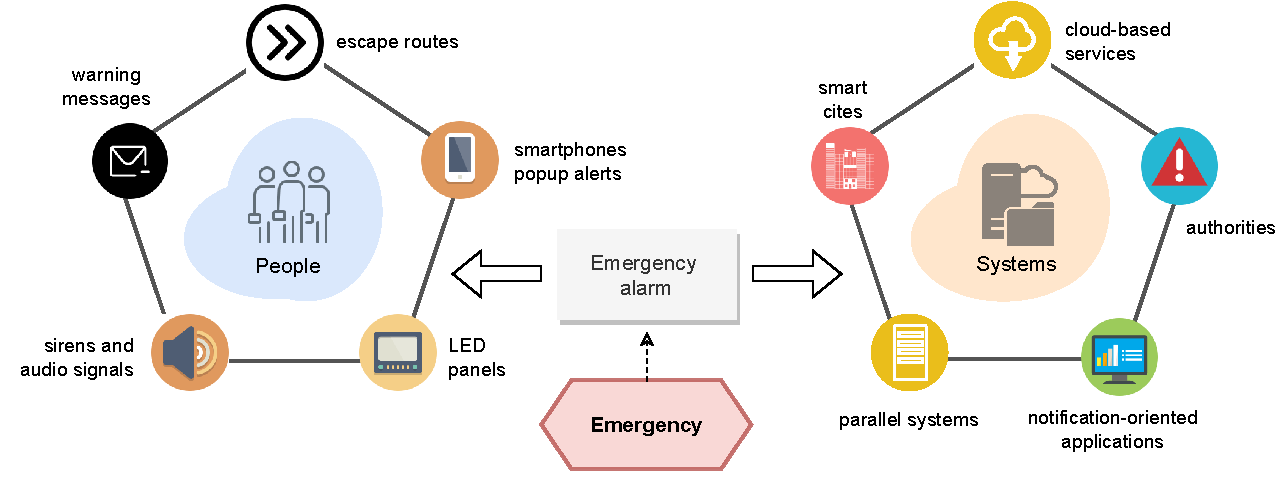
\includegraphics[scale=0.75]{Chapters/1-Survey/images/notifications.pdf}
\caption{Transmitting emergency alarms to different targets in a city.}
\label{Fig:notifications}
\end{figure*}

%%%
\subsection {Alerting affected people}

Directly alerting people has been a major concern when avoiding disasters in cities even before the age of computers, with the implementation of mechanisms to warn all or part of the inhabitants about something potentially dangerous. For example, bells and sirens have been adopted as an affordable and effective way to alert many people in a considerable extensive radius \cite{socialmedia5,citiesemergencies1}. However, notifications can also provide relevant information about the type of an emergency and its intensity, as well as information to guide people to move toward a safer place \cite{emergenciesmetric2}. Additionally, when considering notification strategies, safety plans have been also employed in many localities, with people being previously trained about the procedures to be taken after being alerted about an emergency \cite{quakeculture,citiesdisasters2}. Whatever the case, alerting affected people is a major issue of emergencies management systems, with different particularities to be considered. 

An alerting service is not simply the transmission of emergency alarms. When a person is in the core area of an emergency, she/he will need to receive a very quick and clear emergency alarm since the inflicted damages/injuries might be high. However, people in the neighborhood also need to be alerted, even in a different way. For example, people inside a room where a fire starts will need a more straight alert (e.g. emergency lights in the shape of an arrow pointing to the closest evacuation route), while people in other rooms in the same building may receive notifications in their smartphones indicating how they must orderly exit the building. 

Concerning modern alerting systems, particularly solutions employing IoT technologies, different strategies have been adopted to perform \textit{in loco} notifications. The idea is to alert about emergencies as soon as they are detected in an area, usually employing the same hardware processing units. The work in \cite{iotFire3} monitors fire sources inside a building and alerts people using a LED display to present a safe escape route. In \cite{alertdam1}, sensors are installed over a tailing dam to monitor the flow of debris after an accident, which will trigger flashing lights and sirens along the way to alert people. Since a city may be in the pathway of such flow of debris, this type of emergencies management system may have a deep impact on urban areas. In \cite{iotFire5}, smart exit signs are used to guide people during a fire emergency, changing the displayed information on real-time to update evacuation information. In all these cases, people do not need a gadget or tool to receive notifications, relying on the existing alerting hardware infrastructure. 

Alerting approaches can also directly target people exploiting other resources. In Poland, for example, the Government Centre for Security (GCS) alerts residents about disasters that may threaten their lives \cite{notification2}. After receiving emergency alarms, the GCS sends a notification to mobile network operators, so they can forward the notification to the residents' phones in the threatened area without requiring previous subscription to the service. In a similar perspective, the MyShake platform \cite{iotEarthquake4} considers different sources of data to perform Earthquake Early Warning (EEW), sending notifications to the smartphones of the inhabitants in a potentially affected area. Still considering earthquakes, the work in \cite{notification1} also proposes an EEW system called ShakeAlert that makes use of several seismologic sensors to detect earthquakes as soon as they begin. If some thresholds are exceeded, the system sends notifications to smartphones containing complementary information about the detected earthquake such as origin time, location, magnitude, and extension. 

Although the alerting method should be ubiquitous and quick enough to avoid as much losses as possible, some approaches require manual subscription to a stakeholder. The work in \cite{notification3} presents an early warning system for landslides in Chittagong, Bangladesh. That system makes use of a landslide factor map that describes the risk of landslide in every region of interest. Combining the factor map with weather forecast, the system calculates a risk of landsliding depending on the amount of rainfall that was predicted by the forecasting service. With this information, the early warning system sends e-mail notifications to subscribed stakeholders within 5 days in advance.

Usually, emergencies have been alerted by sirens and other types of audible and visible notifications in the cities. As technology advances and IoT-based devices get cheaper, new methods of alerting have arisen. In the majority of the surveyed works about emergencies alerting targeted at people, mobile messaging was an effective and affordable option, mostly SMS \cite{notification2,notification1,notification4,notification5, notification6} and even audio calls \cite{notification5}. This trend takes advance of the fact that almost every person has a mobile phone on her/his pocket during all day. In fact, it is expected that cellular networks and mobile apps will be of great importance for the development of more efficient emergencies management systems, assuring emergency alerting to many people at low cost. 

%%%
\subsection{Alerting parallel emergency systems}

The direct alerting procedures have the primordial objective of quickly warning people in order to avoid injuries and death. Although this is very reasonable in many cases, the development of more complex emergencies management systems has led to the adoption of modular architectures that separate the services of emergencies detection and alarms notification, which might be provided in a combined or separate way. In the later, alarms are delivered to any requesting system to be further processed, either indirectly forwarding the received alarms to affected people or retransmitting them to other systems.

An important element when delivering generic emergency alarms to other systems is the way data will be processed and formatted. In \cite{emergenciesmetric2,emergenciesmetric3}, emergency alarms are transmitted as JSON (JavaScript Object Notation) messages, organizing metadata in groups of significance. JSON is also adopted in a similar way in \cite{emergenciesmetric5}. For the work in \cite{emergenciesxml}, emergencies scenarios are described in XML (Extensible Markup Language) in a conceptual model for smart cities, which could be structured to represent emergency alarms. The XML formatting standard is also exploited in \cite{emergenciesxml2}, which defines a group of ten-tuple metadata for sensed data that can be easily consulted by other applications to identify emergencies. An extension of XML called CAP (Common Alert Protocol) can also be used to transfer emergency alarms between different systems, as in \cite{notification1}. Actually, the advantage of using formatting standards based on description languages such as JSON and XML is the standardization when describing alarms, allowing easy interaction between systems. Additionally, such languages are based on a flexibility principle when defining the formatting of a group of information, which is highly desired when implementing more complex emergencies management systems.

Other important implementation issue when transmitting generic alarms is the employed transmission paradigm. When considering previous works concerned with emergencies notification, we identified two main transmission paradigms, which are described as follows:

\begin{itemize}
    \item Subscription: When parallel systems want to be notified about emergency alarms, a subscription procedure is taken to register the requesting application. After that, alarms will be synchronously transmitted to all subscribed systems, which will process the received alarms in any possible way. For such transmission paradigm, protocols such as MQTT fit well, as proposed in \cite{emergenciesmetric2,emergenciesmetric3}. For those works, Emergencies Alarm Clients (EAC) subscribe to a MQTT broker to receive generic alarms in real-time. MQTT can also be used to deliver a particular type of emergency alarm, as in \cite{iotFire3,iotmqtt} for fire emergencies. Actually, many solutions based on MQTT have being recently implemented due to the flexibility and easy of use of this subscribe-publish architecture, which can operate over any network protocols. In this sense, many solutions have relied on ZigBee and LoraWAN protocols to assure a wireless transmission infrastructure, with MQTT delivering the emergencies alarms \cite{iotFire3,lora2,iotmqtt2}, assuring low energy consumption and possibly ad hoc transmissions for the considered system;
    
    \item On demand: Some approaches will not require the previous subscription of parallel systems to receive emergency alarms. In such cases, alarms and events-related data are made available in a way that it can be asynchronously accessed. In \cite{emergenciesmetric5}, alarms are saved in a web server to be consulted. In \cite{iotgadget1}, the RESTful architecture is exploited to create web services that provide data about emergency alarms. For \cite{emergenciesxml2}, 
    XML alarms are stored in a NoSQL database do be accessed by any requesting application. In the context of intelligent vehicle systems, the work in \cite{citiesvehicles3} broadcasts warning messages to vehicles in the area where accidents are detected. For such solutions, the nonexistence of a previous subscription process may reduce their overall complexity, although synchronous transmissions in a request-response notification paradigm may increase the time between the detection of an emergency and its proper notification.  
\end{itemize}

Alerting is indeed a vital service in modern emergencies management systems, which should be executed as soon as possible and reaching all affected elements in the area of an emergency. Actually, many approaches will also perform mitigation services in parallel, complementing the transmission of emergency alarms.
`

%%%%%%%%%%%%%%%%%%%%%%%%%%%%%%%%
%%%%%%%%%%%%%%%%%%%%%%
\section {Mitigating emergencies}
\label{sec6}

Although the alerting of people and external systems is a highly relevant objective itself, emergencies management solutions will also want to perform some actions to stop an emergency or even to reduce its negative impacts. Such actions are collectively grouped within the ``mitigation service'', which might ultimately have beneficial implications on the perceived quality of life in modern cities \cite{emergenciesmetric1,smartsensing3}.

Since there are different strategies when mitigating an emergency, the choosing of the best mitigation option concerning timeliness, cost and life preserving has been a major issue. For that, the most common approach has been to associate the nature of the detected emergency with a set of one or more mitigation actions. In this sense, for self-contained emergencies (Section \ref{sec2}), IoT-based solutions have been created to deeply integrate the detection and mitigation of a particular type of emergency, usually combining the operation of sensors and actuators \cite{smartcities2,PlatformsSC}. On the other hand, events-based emergencies have relied on proper definitions of metadata when issuing emergencies \cite{emergenciesmetric2,emergenciesxml2}, which will be leveraged when selecting the most adequate mitigation actions to be taken. In both cases, the nature of the related hazard is of paramount importance, demanding proper understanding of the dynamics of emergencies in urban areas \cite{citiesemergencies1,emergenciesgeneral1}. 

Therefore, emergencies can be mitigated in multiple ways, either directly within the area of incidence of the detected emergency, or even in a broader perspective comprising the dynamics of an entire city. Nevertheless, the evolution of research and development areas such as Internet of Things, Remote Sensing, Big Data and Artificial Intelligence, as well as the continuous maturation of the smart cities paradigm, have significantly changed the way emergencies can be mitigated in a city, improving the efficiency of mitigation approaches when saving lives and reducing properties damages \cite{smartcities1,smartcities2,smartcities3}. This integrated operation is, in fact, one of the promised advantages of smart cities, which puts emergencies mitigation as an inherent service of the cities of the future \cite{smartcities9}. 

Figure \ref{Fig:mitigation} presents an example of how a single emergency of fire can be mitigated in multiple different ways, either locally (triggering sprinklers and shutting down gas distribution in the area) or globally (requesting rescue teams and preparing hospitals to receive victims).

\begin{figure}[ht]
\centering
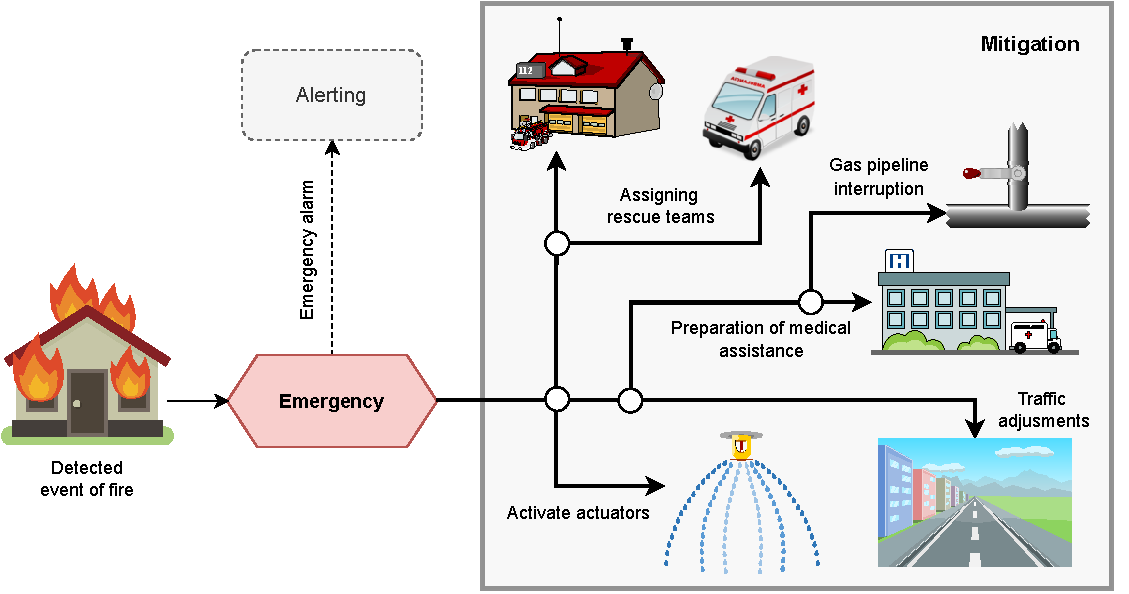
\includegraphics[scale=0.45]{Chapters/1-Survey/images/mitigation.pdf}
\caption{Mitigating a fire-related emergency. Mitigation services may have different objectives and areas of influence.}
\label{Fig:mitigation}
\end{figure}

When surveying mitigation approaches in the literature, it was noticed the adoption of two different strategies. The first strategy is based on direct actions on an emergency in order to cease its existence and to avoid that new emergencies are issued as a consequence of the initially detected emergency. Thus, in this strategy the target is the emergencies and how they can be handled. On the other hand, some works in the literature have been concerned with the impacts of the emergencies, relieving the negative outcomes that emergencies may have on people and properties. Both mitigation strategies have particular challenges in smart cities, being executed separately or in a parallel way, as discussed in next subsections. 

%%%%%%% 1
\subsection{Acting on emergencies}

When wondering about how an emergency can be mitigated in a city, one might say that the best approach is to fight the cause of that emergency. Actually, this is a very reasonable idea, since it has been the most usual approach when fighting emergencies in centuries \cite{fireevolution,firetemporaldata1}. With the advent of IoT technologies and sensor and actuator networks, such actions could be automatized in different ways, opening a new era of possibilities for emergencies mitigation in smart cities. 

Many automatized mitigation services have been proposed lately, employing different hardware components according to the type of emergencies to be mitigated. Actually, some proposed approaches are centered around one or more types of emergencies, which will dictate the type of actuators that will be more effective to mitigate a particular emergency. This fact can be seen in Table~\ref{Tab:mitigation}, which summarizes some works with these characteristics. 

\begin{table}
    \centering
    \caption{Some IoT-based approaches to directly act on emergencies in smart cities.}
    \label{Tab:mitigation}
    \begin{tabular}{|c|c|c|}
        
        \hline
        \textbf{Work} & \textbf{Emergency} & \textbf{Actions} \\
        
        \hline
        \citeauthor{mitigationAct1} \cite{mitigationAct1} & fire       & activate sprinklers \\

        \hline
        \citeauthor{iotEarthquake2} \cite{iotEarthquake2} & earthquake & turn off electricity, gas and water \\

        \hline
        \citeauthor{SultanMahmud2017} \cite{SultanMahmud2017} & fire   & turn off electricity, activate sprinklers \\

        \hline
        \citeauthor{iotFlood2} \cite{iotFlood2} & flood & open dam gates according to the water level \\
        
        \hline
        \citeauthor{mitigationAct3} \cite{mitigationAct3} & fire       & turn off electricity, release extinguishing gases \\

        \hline
        \citeauthor{mitigationAct4} \cite{mitigationAct4} & fire       & activate a water spray \\

        \hline
        \citeauthor{mitigationurban7} \cite{mitigationurban7} & fire       & dispatch drones do drop fire extinguishing balls \\

        \hline
        \citeauthor{mitigationAct6} \cite{mitigationAct6} & smoke       & activate smoke extraction fans \\

        \hline
        \citeauthor{mitigationAct7} \cite{mitigationAct7} & flood       & control watershed gates \\

    \end{tabular}
\end{table}

When acting on emergencies exploiting sensors and actuators, some interesting considerations can be taken. While works like \cite{SultanMahmud2017} and \cite{mitigationAct1} are intended to cease the cause of an emergency, directly facing the original hazard, the work in \cite{iotEarthquake2} can not avoid the issued emergency, but it can prevent the issuing of new emergencies derived from the original one. The same is true when adjusting traffic lights after an accident in order to avoid additional accidents \cite{mitigationITS1,rego2018software}. In all these cases, although the outcomes may be different, the employed approach will directly act on the issued emergencies.

Other important remark is about the level of automation in the implemented systems. In \cite{iotFlood2}, for example, sensors are used to monitor the level of dams, sending information to a data processing center. However, the decision of opening dam gates is made by personnel after analyzing the retrieved sensed data. Such human-assisted decisions are not rare since they may be valuable in some scenarios when the risks involved are too high \cite{humanAssisted1}.

%%%%%% 2
\subsection{Relieving emergencies}

The mitigation strategy for a group of approaches will be to relieve the impact that emergencies may have on people and the infrastructure of a city, reducing injuries, deaths and economical losses as good as possible. For that, an integrated perspective of a city is usually required, since such relief will depend on other services provided in a smart city context. As an example, while a mitigation service dedicated to act on a fire will try to extinguish it, a relieving strategy will contact an external system responsible for rescuing and firefighting in order to request the dispatching of ambulances and fire trucks toward the affected area. With the maturation of smart cities, more integrated solutions have emerged, promising more efficient support to emergency situations. 

When an emergency is detected in an area, the city may respond to facilitate the arrival of rescue teams and eventual supplies. Actually, fast arrival of rescue teams are critical during an emergency \cite{mitigationurban3}, which have fostered important research developments in this area. In \cite{mitigationurban1}, a logistics distribution approach is proposed to create a fast supply network toward affected areas, which may be created to last for longer than the expected duration of an emergency (e.g. when there is a perception that the emergency is turning into a disaster). Such approach, which comprises fuzzy-based decisions in a macro designing of a city, would be valuable before the dispatching of emergency vehicles such as ambulance and fire trucks, adjusting routes and potential relief areas. Similarly, the work in \cite{mitigationurban3} proposes a large-scale solution to support the mitigation of emergencies during a flood situation, specially focused in the accessibility of response teams. Since surface water and fluvial flooding may delay response teams during an emergency, multiple types of data in a city are considered to define optimal routing maps that should be taken by rescue teams in such conditions.

In several situations, first responder vehicles such as ambulances, fire trucks and police cars need to get to the emergency area as soon as possible. Since traffic can be jammed in large cities, some authors have proposed traffic management and signaling solutions in emergency situations. The work in \cite{mitigationurban4} is aimed at reducing the travel time of emergency vehicles during a mitigation process. In order to avoid wasted time due to red light signals, the authors proposed Arduino managed traffic lights. This way, the lights on the streets are managed by Arduino boards connected to the Internet that can receive commands from an Android application used by an emergency vehicle co-driver. That app can then be used to turn lights green in a way that the total travel time is reduced. However, while the work in \cite{mitigationurban4} requires manual intervention using an app, the authors of \cite{mitigationurban5} developed a semi-automatized approach that takes into consideration the current traffic in the city and also sets different priorities for emergency vehicles. A Central Traffic Controller (CTC) assigns movement priorities after gathering metadata of the issued emergencies, sending the routes to each emergency vehicle considering the current traffic conditions. With a GPS device in the vehicles, the CTC can get their position in real-time and then manipulate traffic lights directly. In a more automatized way, the work in \cite{rego2018software} divides a smart city into clusters comprised with smart traffic lights and electronic signaling. Once an emergency is detected, the system sends a message through the defined network asking for resources and informing the smart lights and signals how to operate to modify the traffic accordingly. When the emergency finishes, the system sends another message informing the lights and signals to resume their normal operations. 

Macro perceptions of traffic in a city are highly desired although the implemented solutions may become too complex. As an example, authors in \cite{s150614370} proposed a smart signaling system to inform users (citizens, drivers, etc.) of emergency situations. A system of connected sensors monitors the environment inside a tunnel and detects a fire situation, allowing the determination of the best exits according to the position of the fire source and smoke conditions. Then, smart signals are settled accordingly, directing the users to a safe exit.

Another problem related to emergency vehicles is the (automatic) assigning of rescue teams according to the type of the detected emergencies and their metadata. The work in \cite{costa2020automatic} proposes an emergency vehicles assignment algorithm according to the issued emergencies, selecting the most appropriate vehicles in a city that is experiencing multiple concurrent emergencies in different areas. In that work, the expected negative impact of each current emergency is assessed, being combined with the distance from the available emergency vehicles to the area of incidence of each emergency. The combined result of these parameters is then used to assign the most effective (and potentially closer) emergency vehicles. For the work in \cite{mitigationurban2}, sensed data are transmitted to a central unit to be processed along with other data. Then, issued emergencies are coordinately answered by mitigation actions, with the assignment of polices, firefighters or medical staffs teams according to the type of the issued emergencies. 

Relieving mitigation actions can also come from the sky. In \cite{emergencyRescue3}, camera-enabled drones are expected to support in rescue operations, identifying the number and the locations of victims in a building. For the work in \cite{mitigationurban6}, drones equipped with cameras are also considered to support rescue teams when identifying victims. In \cite{mitigationAct5}, drones are used to ``mark'' critical areas that need assistance during an emergency. In all these cases, drones are an important supportive resource, but they can also be used in different ways. In \cite{mitigationurban8}, drones are dispatched as a first response to an emergency call in order to provide initial information for the victims. Actually, when adopting microphones or even LEDs, drones can be a very fast response resource during emergencies, reaching areas that vehicles can not go. In fact, this perspective could be seen during the COVID-19 pandemic, with drones supporting social distancing measures \cite{dronecovid1} and sanitation \cite{dronecovid2}.  


%%% 7 %%%%%%%%%%%%%%%%%
%%%%%%%%%%%%%%%%%
\section{Open challenges and future directions}
\label{sec7}

The development of emergencies management systems have to deal with a lot of aspects related to the modelling of emergencies, the detection of emergencies, the transmission and displaying of warning messages, and the mitigation of emergencies in cities. These major concepts were surveyed and discussed in this article, giving important clues about important development issues and evolution trends in this complex area. However, although a comprehensive perception of the state-of-the-art in this complex subject has been provided in this article, some open challenges and future directions still need to be discussed, potentially supporting research efforts in the coming years.

\subsection{Technologies and development trends}

Roughly speaking, although technological aspects are highly relevant when implementing emergencies management systems in the era of internet of things, artificial intelligence and smart vehicles, this area is still evolving and new technological tools are constantly being developed. Actually, it is reasonable to expect that sensors-based systems and IoT devices will still drive the development of emergencies management systems, but their maturation will depend on new innovative ideas for the emerging challenges to be presented.

An important development trend is the utilization of low-power affordable miniaturized hardware to support in the detection, alerting, and mitigation of emergencies. Obviously, since each of these phases have particular challenges, as discussed in this article, such hardware is expected to be embraced in different ways. Notably, a recent trend has been to endow such hardware units with Machine Learning algorithms adapted to processing, memory, and energy constraints. This resulting TinyML paradigm should be one of the flagships for the new generation of emergencies management systems. 

The TinyML concept is highly suitable to the edge computing paradigm, which is another important development trend. Scattering the processing burden, more complex computations could be performed to allow the issuing of more complex aggregated emergencies. Since the smart cities environment is naturally prone to the execution of multiple parallel systems, the availability of multiple data source could be exploited by the computing on the edge, potentially leading to the quick execution of detection and response procedures. In our opinion, this is a promising development trend to be followed.

In parallel, recent works have started to develop soft sensors approaches to tackle the particular problems of smart cities \cite{softsensor,softsensor3}, virtually creating a layer of sensors with more complex (and abstract) data. Since soft sensors provide new types of data combing input data from sensors and other data sources, emergencies detection can directly benefit from this idea. Moreover, when TinyML is combined with the principle of soft sensors \cite{softsensor2}, more efficient EDUs could be designed at affordable prices. Future works in this area should then bring some breakthroughs for the development of emergencies management systems.

Besides the presented trends, other technological innovations that better support the development of cyber-physical systems in the context of smart cities should favor the maturation of emergencies management systems. We believe such hardware-software integration should be the cornerstone for new developments in this area.

%%
\subsection{Urban inequalities and smart solutions}

The urban sprawl since the initial industrial revolution has considerably changed the landscape of humankind, with large cities emerging in all continents and transforming our way of living. In this new environment, many inherent problems of large cities have driven research and development efforts in last decades, with challenges related to urban mobility, sanitation, pollution and energy efficiency encompassing major concerns. However, with the development of new technologies, the safety and well-being of the cities inhabitants have come to the table, which may significantly benefit the quality of life in urban areas.

Overall, smart cities have been promoted as a way to improve urban livability, becoming almost common sense that smarter cities are naturally better \cite{citylife}. However, since cities still have different social-economic organizations, many people may not have fair access to the cities resources, smart or not \cite{inequalities1}. Actually, some of the initially developed services in the smart cities trend were focused on efficient public lightning and traffic efficiency, which have been mostly implemented in richer areas of the cities that already had better urban infrastructure \cite{inequalities3}. A similar pattern can be perceived when considering the popular bike sharing service and the availability of greener public mobility alternatives \cite{smartcycling}. In fact, if not planned considering the general public interest, many smart cities solutions may become tools to increase social and economic inequalities. 

When coming to emergencies management systems, ``how'' has been a highly recurrent question that have driven most research efforts lately. However, ``where'' should also be a major concern, since the detection, alerting, and mitigation of emergencies should be provided regardless of socio-economic configurations and the pressures of the real state market. This concern should be more evident in this transition process from ``traditional'' cities to smart cities, mostly because the (initially) limited resources will eventually raise questions about which populations should be given priority in the allocation of such resources. 

It can be said that social vulnerability, population density, rescuing difficulties and potential of damage are some of the questions that should be answered before assuming that richer areas deserve better coverage by emergencies management systems \cite{emergenciesmetric1}. Therefore, considering the development patterns of large cities in the last centuries, fair access to smart cities services should remain an important challenge to be faced. 

%%%%%%%%%%%%%%%%%%%
\subsection{Infectious diseases as emergencies}

In 2020, a pandemic hit the entire globe within a relatively short amount of time. Due to fast well-connected transportation networks, the COVID-19 virus rapidly spread, leading to lockdowns and dramatically interrupting international trade routes and people circulation. In a sudden, our urban way of life facilitated the dissemination of the SARS-CoV-2 virus in a scale never seen before in the human history, raising a lot of questions about how the humankind can be prepared for the next pandemics.

The COVID-19 was the fist large pandemic that was faced in the era of smart cities. The state-of-the art in monitoring technologies, distributed databases and artificial intelligence algorithms could be put on service to track suspicious cases, to predict new infections and even to prepare hospitals to attend sick people. However, although the obtained results were significant when compared with the adopted measures in previous pandemics, the employed solutions were mostly punctual cases. Actually, with the maturation of smart cities and the consequent larger integration among systems, the full potential of health-centric services to predict, detect and isolate new infections might be achieved \cite{covidsmartcities2}.

Even after proper vaccination and the substantial reduction in the number of COVID-19 cases and deaths, it is reasonable to say that the post-pandemic world will be deeply impacted by the use of new technologies in public and private spaces. And this scenario, which will be naturally more prone for the adoption of distributed smart applications, will dictate how cities will evolve henceforth. As a result, smart cities initiatives are expected to be promoted more intensively in the coming years \cite{covidsmartcities6}.

Roughly speaking, the spread of a modern infectious disease can be perceived as a urban emergency \cite{covidsmartcities1}. This way, detection, alerting, and mitigation actions can be performed to handle an infectious disease outbreak or even a pandemic. Therefore, all previously discussed subjects and approaches could be leveraged to prevent or even to slow down a virus spreading. Particularly, some works have already focused on this matter, for example the work in \cite{twitter2} that uses the Twitter social media to detect an outbreak. Thermal cameras and image processing algorithms were also largely used during the COVID-19 pandemic to detect fever and potentially infected individuals \cite{covidsmartcities4}, and thus such technologies should still be used as standard tools. However, since a pandemic has a very wide perspective considering numerous aspects, comprising not only health assistance but also indirect services such as public transportation, the inherent integrated nature of smart city services might play an important role when detecting and even preventing next pandemics. For the evolving emergencies management systems, the next pandemic should always be a concern.

%%
\subsection{Smart cities development and integration}

A practical challenge for efficient emergencies management is the integration among the different systems within a smart city environment. Actually, most smart cities in the last decade have been developed as independent services with a well-defined set of objectives and input data. In this sense, cities around the world have seen some initiatives being developed and implemented as a practical service for the inhabitants \cite{citiestransforming,citiestransforming2}, but the actual integration among them is still in initial steps. The next generations of smart cities should then be devoted to such integration \cite{smartcities3}, which could not only incorporate the emergencies management service but also provide valuable data to support the detection, alerting, and mitigation of emergencies.

The smart city systems that are already being developed may present some opportunities for the evolution of emergencies management systems. The following are some of them \cite{citiestransforming}:

\begin{itemize}
    \item Smart healthcare: data provided by hospitals are valuable for different mitigation actions, specially when informing about the number of available ICU beds and the current configurations of medical assistance teams. During an emergency, such data provided by these parallel systems could indicate the best options when injured people need immediate assistance. When concerning ambulances, their number, location and current occupation is also relevant for mitigation actions: after an emergency is detected, the emergencies management system may send a request to the the smart healthcare system for the quick dispatching of ambulances to an affected area, taking all emergencies' metadata into account;
    
    \item Intelligent transportation systems: the way vehicles and public transportation will behave in a city may also be integrated to the management of emergencies. In this sense, not only traffic accidents detected by the traffic system may be forwarded to an emergencies management system, but also the traffic infrastructure may be adapted to deal with an ongoing emergency in a city. Actually, some recent works have already proposed some solutions in this area, but a deeper integration between both services may improve the achieved results. In this trend, we expected that Vehicular Networks (VANET) will become more popular and ubiquitous, with a higher potential for integration with other systems.

    \item Smart security: public security systems may also provide valuable data for the perception of emergencies, specially when considering urban hazards. Moreover, the existing infrastructure of cameras can be leveraged to enhance the detection capacity of emergencies management systems. In such integration, the monitoring resources in a city may be increased, even considering different objectives. As an additional trend, police vehicles may also be dispatched by a smart security system under request, which is in fact an important component of mitigation actions during an emergency;
    
    \item Smart environment monitoring: current monitoring systems that employ fixed sensors stations, drones and even remote sensing through satellites are becoming very common in many cities, providing not only a more accurate forecast but also alerting about potential dangerous weather conditions. Many of such systems already have emergencies detection capabilities, although they operate within a well-defined context. Hence, an integration could enhance the efficiency of emergencies management systems, while reducing the associated costs when already deployed sensors are concurrently used by both systems.
\end{itemize}

These and other potential integration among two or more smart city systems will have to deal with some integration challenges, demanding common interfaces. Since integration issues are also relevant in other smart cities contexts, some works have already addressed the development of smart cities systems that comply with defined standards \cite{snap4city,validation1}. In fact, validation of future proposed systems will be always an important design issue, with methodologies, evaluation labs, and supportive tools emerging to address this matter. Overall, we believe this will be one important development trend for emergencies management systems.

%%%%%%%%%%%%%%%%%
\section{Conclusions}
\label{conclusion}

For the development of more sustainable and resilient cities, emergencies should be treated as one of the main elements of the urban dynamics, potentially affecting multiple systems in a city environment. Actually, with most world population living in urban areas, with increasingly presence of large and mega cities, the negative impacts of emergencies and disasters have been more significant in the last decades. This scenario has fostered the adoption of different emergency-prone approaches in multiple contexts, but the challenges imposed by overcrowded cities will still demand more efficient solutions.

This article addressed technological issues of hardware, software, data, and networking related to emergencies management systems in urban scenarios. After the performed discussions, classifications and analyses, a comprehensive snapshot of this research area was obtained, potentially supporting a deeper understanding of its state-of-the-art.

As could be seen, smart cities will handle emergencies through detection, alerting, and mitigation services, which will be based on well-defined models and data formats. Although many solutions have been developed to address specific problems, as discussed in this article, it was perceived that a natural trend is to develop more integrated solutions, treating the city as a broader system with highly interconnected subsystems. This principle should be more often considered in future works. 

In general, detection, alerting, and mitigation are the pillars of emergencies management systems. Nevertheless, other important research subjects are also relevant and should be also considered when developing more efficient smart solutions for current and future emergencies, for example comprising research topics such as networking, security, energy efficiency, availability, among others. Since this whole research area is very active, with many new solutions still emerging in the coming years, very creative solutions integrating existing and new technologies should be proposed, bringing promising results.

% \bibliographystyle{unsrtnat}
% \bibliographystyle{abnt-alf}
% \bibliography{Chapters/1-Survey/references}

\printbibliography[heading=subbibliography]
\end{refsection}